\documentclass{llncs}% ===> this file was generated automatically by noweave --- better not edit it
\usepackage{draftwatermark}
\SetWatermarkLightness{0.95}
\usepackage[utf8x]{inputenc}
\usepackage[colorlinks=true,urlcolor=blue,linkcolor=blue,citecolor=blue]{hyperref}
\usepackage{fourier}
\usepackage{tikz}
\usetikzlibrary{arrows,automata}
\usepackage{marvosym,alltt}
\usepackage{graphicx}
\usepackage{amsmath}
\usepackage{upgreek}
\usepackage{bbm}

\usepackage{listings}
\definecolor{LtGray}{rgb}{0.95,0.95,0.95}

\lstset{
%\lstdefinestyle{maude}{%
basicstyle=\scriptsize, % the size of the fonts that are used for the code
columns=fullflexible,
mathescape=true,
tabsize=2, linewidth=\columnwidth, 
numbers=left,                           % where to put the line-numbers
numberstyle=\tiny,                      % the size of the fonts that are used for the line-numbers
stepnumber=1,                           % the step between two line-numbers. If it's 1 each line will be numbered
numbersep=5pt,                  % how far the line-numbers are from the code
backgroundcolor=\color{LtGray},% choose the background color. You must add \usepackage{color}
showspaces=false,                       % show spaces adding particular underscores
showstringspaces=false,         % underline spaces within strings
showtabs=false,                 % show tabs within strings adding particular underscores
frame=lines,                            % adds a frame around the code
tabsize=2,                                      % sets default tabsize to 2 spaces
captionpos=b,                           % sets the caption-position to bottom
floatplacement={tbp},
breaklines=true,                        % sets automatic line breaking
breakatwhitespace=false,                % sets if automatic breaks should only happen at whitespace
escapeinside={\%*}{*)},         % if you want to add a comment within your code
numberbychapter=false,
}

\lstdefinelanguage{maude}{ keywords={pr, ex, inc, fmod, endfm, mod,
    is, endm, sort, sorts, subsort, op, ops, eq, rl, ceq, if, then,
    else, fi, crl, assoc, comm, ctor, id, var, vars, mb, cmb, view, endv, to, format} }
\lstnewenvironment{maude}[1][]{\lstset{language=maude,#1}}{}

\usepackage{noweb}

% Comandos do noweb:
% noweave -delay bplc.noweb > bplc.tex
% notangle -Rbplc.maude bplc.noweb > bplc.maude 

\renewcommand{\date}{\today}

\begin{document}
        
\title{$\uppi$ Framework}
\author{Christiano Braga\\\email{cbraga@ic.uff.br}}
\institute{Instituto de Computação\\Universidade Federal Fluminense}

\maketitle

\begin{center}
\date
\end{center}

%\begin{center} 
\includegraphics[scale=0.45]{../logo/logo.png}\end{center}


\begin{abstract}
$\uppi$ framework is comprised by $\uppi$-lib, a library of common programming language constructs whose semantics are formally specified, and $\uppi$-automata, an au\-to\-mata-based formalism to describe the operational semantics of programming languages.  To give semantics to a programming language means to relate constructions of the given language with the constructs of $\uppi$-lib. It is implemented in the~\href{http://maude.cs.uiuc.edu}{Maude} language.
\end{abstract}

\pagestyle{plain}

\section{Introduction}

The $\uppi$ framework is comprised by $\uppi$-lib, a set of programming languages constructs inspired by Peter Mosses' Component-Based Semantics~\cite{Mosses:2008:CDP:2227536.2227559} and $\uppi$-automata, an au\-to\-mata-based formalism to describe the operational semantics of programming languages, that generalizes Gordon Plotkin's Interpreting Automata approach~\cite{plotkin}.   
Since $\uppi$-lib has an automata-based semantics, $\uppi$-lib programs can be model checked or be subjected to any automata-based validation technique. The Maude~\cite{Clavel:2007:MHL:1808998} implementation of $\uppi$-lib\footnote{\url{http://github.com/ChristianoBraga/BPLC}} allows for rewriting-based execution, Linear Temporal Logic model checking and narrowing-based symbolic execution of $\uppi$-lib programs. 

This report describes $\uppi$, an automata-based semantic framework for teaching formal compiler construction and its implementation in the Maude language. From a pedagogical perspective, being automata-based helps closing the gap between compiler construction and subjects such as Introduction to Programming Languages, Programming Languages Semantics and Formal Languages and Automata Theory, that usually precedes Compiler Construction courses. Our previous experience with the formal specification of programming languages, in particular the component-based framework, helped us devise an approach of operational character that formalizes a core (or intermediate) language amenable to automated verification and code generation. 
%The proposed semantic framework is a result of a long term
%collaboration with FC, EHH, JM and PDM. The influence of PDM's work on
%modular semantics and component-based semantics, together with
%Rewriting Logic and Maude is fundamental. $\uppi$-lib is a ``fork'' of
%component-based semantics and the characteristics of the Term
%Rewriting System associated with a Generalized Interpreting Automata
%were found by many years of work with Rewriting Logic, the Maude
%system and collaboration to the Rewriting Logic Semantics project~\cite{MESEGUER2007213}.

The remainder of this report is organized as follows. Section~\ref{sec:preliminaries} recalls some preliminary material to the discussion of $\uppi$-automata, subject of Section~\ref{sec:gia}. The $\uppi$-automata semantics of $\uppi$-lib is discussed in Section~\ref{sec:uppi-lib-sig}, together with its Maude implementation and the \textsc{Imp} compiler. 

\section{Preliminaries}\label{sec:preliminaries}

Before introducing the $\uppi$ framework and its Maude implementation we first recall, in Section~\ref{sec:pre-os}, some basic concepts from operational semantics and model checking and, in Section~\ref{sec:pre-maude}, the Maude language.

\subsection{Transition systems, structural operational semantics and model checking}\label{sec:pre-os}

This Section recalls, very briefly, just for completeness, the basic concepts of labeled and unlabeled transition systems, structural operational semantics and model checking.

A labeled transition system~\cite{arnold1994finite} (LTS) is a tuple $\mathcal{T} = (S, \rightarrow, L)$, where $S$ denotes the set of the states of the system, $\rightarrow \subseteq S \times L \times S$ is the transition relation, with $L$ a set of labels. An unlabeled transition system is an LTS where $L = \emptyset$. A concurrent system may have labeled transition systems as models, with $L$ denoting the set of actions of the system, that may eventually synchronize. 

Labeled transition systems are the standard models of structural operational semantics descriptions. Given an SOS description $\mathcal{M} = (G, R)$ specifying the semantics of a programming language $L$, the set $G$ defines the grammar of $L$ while relation $R$ represents the semantics of $L$ (either static or dynamic) in a syntax-directed way.   
Equation~\ref{eq:sos-congr} presents the general form of the (unlabeled) rule for 
the inductive step of the evaluation of a programming language
construct $f$ in the SOS framework, where $\rho$ and $\rho'$ are environments, $\rho'$ is the result of
some computation involving $\rho$, $f$ is programming language
construct and $t_i$ its parameters,
$\sigma, \sigma', \sigma_i, \sigma'_i$ are memory stores, with
$\sigma'$ the result of some computation of $\uplus^n_{i=1}\sigma'_i$, and
$\mathit{Cnd}$ is a predicate not involving transitions.
\begin{equation}\label{eq:sos-congr}
\frac{\rho' \vdash \bigwedge^n_{i=1} t_i, \sigma_i \Rightarrow t'_i, \sigma'_i}
     {\rho \vdash f(t_1, t_2, \ldots, t_n), \sigma
       \Rightarrow f(t'_1, t'_2, \ldots, t'_n), \sigma'} \mbox{ if } \mathit{Cnd}
\end{equation}
Typically, SOS rules have a \emph{sequent} in the conclusion of the form $\rho \vdash g , \sigma \Rightarrow g' , \sigma'$, where $g$ and $g'$ are derivations of $G$. If one looks at the conclusion as a transition of the form $(\rho, g, \sigma) \Rightarrow (\rho, g', \sigma')$ than the construction of the (unlabeled) transition system $\mathcal{T}$ from $\mathcal{M}$ becomes straightforward with $(\rho, g, \sigma) \in S$.

Model checking~\cite{Clarke:2000:MC:332656} is an automata-based automated validation technique to solve the ``question'' 
$\mathcal{T}, s \models \varphi$, that is, does model $\mathcal{T}$, a transition system, or Kripke structure in Modal Logic~\cite{goldblatt} jargon, with initial state $s$, satisfies property $\varphi$? The standard algorithm checks if the language accepted by the intersection B\"uchi automaton (a regular $\Omega$-automaton, that is, an automaton that accepts infinite words) of $\mathcal{T}$ and $\neg\varphi$ is empty.  

\subsection{Maude}\label{sec:pre-maude}

In this Section we introduce the main elements of the Maude language, our choice of programming language for this work. 

The Maude system and language~\cite{Clavel:2007:MHL:1808998} is a high-performance implementation of Rewriting Logic~\cite{meseguer92}, a formalism for the specification of concurrent systems that has been shown to be able to represent quite naturally many logical and semantic frameworks~\cite{marti-oliet-meseguer:2002}.

Maude\footnote{Maude allows for programming with different Equational Logics: Many-sorted, Order-sorted or Membership Equational Logic. In this paper, Maude programs are described using Order-sorted Equational Logics.}
is an algebraic programming language. A program in Maude is organized by modules, and every module has an initial algebra~\cite{Goguen:1996:ASI:547173} semantics. Module inclusion may occur in one of three different \emph{modes}: \texttt{including}, \texttt{extending} and \texttt{protecting}. The \texttt{including} mode is the most liberal one and imposes no constraints on the preservation of the algebra of the included module into the including one, that is, both ``junk''  and ``confusion''\footnote{Informally, when ``junk'' may be added  to an algebra but ``confusion'' may not, as in \texttt{extending} mode, it means that new terms may be included but are not identified with old ones.} may be added. Inclusion in \texttt{extending} mode may add ``junk'' but no ``confusion'', while inclusion in \texttt{protecting} mode adds no ``junk'' and no ``confusion'' to the included algebra. Module inclusion is not enforced by the Maude engine, being understood only as an indication of the intended inclusion semantics. Such declarations, however, are part of the semantics of the module hierarchy and may be important for Maude-based tools, such as a theorem prover for Maude specifications, that would have to discharge the proof obligations generated by such declarations. 

Computations in Maude are represented by rewrites according to either equations, rules or both in a given module. Functional modules may only declare equations while system modules may declare both equations and rules. Equations are assumed (that is, yield proof-obligations) to be Chruch-Rosser and terminating~\cite{Baader:1998:TR:280474}. Rules have to be coherent: no rewrite should be missed by alternating between the application of rules and equations. 
A (concurrent) system is specified by a rewrite system $\mathcal{R} = (\Sigma, E \cup A, R)$ where $\Sigma$ denotes its signature, $E$ the set of equations, $A$ a set of axioms, and $R$ the set of rules. The equational theory $(\Sigma, E \cup A)$ specifies the states of the system, t terms in the $\Sigma$-algebra modulo the set of $E$ equations plus $A$-axioms such as associativity, commutativity and identity. Combinations of such axioms give rise to different rewrite theories such that rewriting takes place modulo such axioms. Rules $R$ specify the (possibly) non-terminating behavior, that takes place modulo the equational theory $(\Sigma, E \cup A)$. 
Another interesting feature of Maude is to support \emph{non-linear patterns} (when the same variable appears more than once in a pattern) both in equations and rules. Section~\ref{sec:gia-in-maude} exemplifies how this feature is intensively used in the Maude implementation of the $\uppi$-automata framework.

An interesting remark regards the decision between modeling behavior as equations or rules.  One may specify (terminating) system behavior with equations. The choice between equations and rules provides an \emph{observability gauge}. In the context of a software architecture, for instance, \emph{non-observable} (terminating) actions, internal to a given component, may be specified by equations, while \emph{observable} actions, that relate components in a software architecture, may be specified as rules.  Section~\ref{sec:gia-in-maude} illustrates how this ``gauge'' is used in the Maude implementation of the $\uppi$ framework.  

A compiler can be implemented in Maude as a \emph{meta-level} application. Such a Maude application uses the so called \emph{descent functions}~\cite[Ch.11]{maude} that represent modules as terms in an \emph{universal} theory, implemented in Maude as a system module called META-LEVEL. Some of the descent functions are metaParse, metaReduce, metaRewrite and metaSearch. Function metaParse receives a (meta-represented) module denoting a grammar, a set of quoted identifiers representing the (user) input and a quoted identifier representing the rule that should be applied to the given input qids, and returns a term in the signature of the given module. Descent function metaReduce receives a (meta-represented) module and a (meta-represented) term and returns the (meta-represented) canonical form of the given term by the exhaustive application of the (Church-Rosser and terminating) \emph{equations}, only, of the given module.  A interesting example of metaReduce is the invocation of the model checker at the metalevel: (i) first, module MODEL-CHECKER must be included in a module that also includes the Maude description of the system to be analyzed, and (ii) one may invoke metaReduce of a meta-representation of a term that is a call to function modelCheck, with appropriate parameters, defined in module MODEL-CHECKER. Finally, function metaRewrite simplifies, in a certain number of steps, a given term according to both equations and rules (assumed coherent, that is, no term is missed by the alternate application of equations and rules) of the given module. Meta-search looks for a term that matches a given \emph{pattern}, from a given term, according to a choice of rewrite relation from $\Rightarrow^*$, $\Rightarrow^+$, $\Rightarrow^!$, denoting the reflexive-transitive closure of the rewrite relation, the transitive closure of the rewrite relation or the rewrite relation that produces only canonical forms.

Section~\ref{sec:gia} continues this paper by introducing $\uppi$-automata.

\section{$\uppi$-automata}\label{sec:gia}

\subsection{Interpreting automata}

%An Interpreting Automata is a decision device that accepts a language
%by interpreting string (commands) on a control stack in the context of a memory
%store and a value stack. 
In~\cite{plotkin}, Plotkin defines the concept of Interpreting Automata as finite-state Transition Systems as a semantic framework for the operational semantics of programming languages. Interpreting Automata are now recalled from the perspective of Automata Theory.

Let $\mathcal{L}$ be a programming language accepted by a Context Free Grammar (CFG) $G = (V, T, P, S)$ defined in the standard way where $V$ is the finite set of variables (or non-terminals), $T$ is the set of terminals, $P \subseteq V \times (V \cup T)^*$ and $S \not\in V$ is the start symbol of $G$.
An Interpreting Automaton for $\mathcal{L}$ is a tuple $\mathcal{I} = (\Sigma, \Gamma, \rightarrow, \gamma_0, F)$ where $\Sigma = T$, $\Gamma$ is the finite set of configurations, $\rightarrow \subseteq \Gamma \times \Gamma$ is the transition relation, $\gamma_0 \in \Gamma$ is initial configuration, and $F$ the finite set of final configurations. Configurations in \(\Gamma\) are triples of the general form
\[
\Gamma = \mathit{Value~Stack} \times \mathit{Memory} \times \mathit{Control~Stack}.
\]
where $\mathit{Value~Stack} = L(G)$ with $L(G)$ the language accepted by $G$, the set
\(\mathit{Memory}\) is a finite map \(\mathit{Var}
\to_{\mathit{fin}} \mathit{Storable}\) with $\mathit{Var} \in V$ and $\mathit{Storable} \subset T^*$, and the elements of the
$\mathit{Control~Stack} = L(G) \cup \mathit{KW}$, where $\mathit{KW}$ is the set of keywords of $\mathcal{L}$. 
A computation in $\mathcal{I}$ is defined as $\rightarrow^*$, the reflexive-transitive closure of the transition relation.

As an example, let us consider a programming language $\mathcal{L}$ with arithmetic expressions,
Boolean expressions and commands with the CFG in Figure~\ref{fig:l-cfg}.
\begin{figure}
\[
\begin{array}{rcl}
\mathit{Prog} & ::= &  \mathit{ComSeq} \\
\mathit{ComSeq} & ::= & \mathtt{nop} \mid \mathit{Com} \mid \mathit{Com} ~\mathtt{;}~ \mathit{ComSeq}   \\
\mathit{Com} & ::= & \mathit{Var} ~\mathtt{:=}~ \mathit{Exp} \mid \\
                     &  & \mathtt{if}~ \mathit{BExp}~ \mathit{ComSeq}~ \mathit{ComSeq} \mid \\
                     &  & \mathtt{while}~ \mathit{BExp}~ \mathit{ComSeq} \\
\mathit{Exp} & ::= & \mathit{BExp} \mid \mathit{AExp} \\
\mathit{BExp} & ::= & \mathit{Exp} ~\mathit{BOP}~ \mathit{Exp} \\
\mathit{BOP} & ::= & \mathtt{=} \mid \mathtt{or} \mid \mathtt{∼} \\  
\mathit{AExp} & ::= & \mathit{AExp} ~\mathit{AOP}~ \mathit{AExp} \\
\mathit{AOP} & ::= & \mathtt{+} \mid \mathtt{-} \mid \mathtt{*} 
\end{array}
\]
\caption{CFG for $\mathcal{L}$}\label{fig:l-cfg}
\end{figure}

The values in the $\mathit{Value~Stack}$ are
elements of the set 
$\{\mathbbm{T} \cup \mathbbm{N} \cup \mathit{Var} \cup \mathit{BExp} \cup \mathit{Com},$ 
where \(\mathbbm{T}\) is the
set of Boolean values, \(\mathbbm{N}\) is the set of Natural numbers,
with \(\mathit{Var}\) the set of variables, \(\mathit{BExp}\) the set
of Boolean expressions, and \(\mathit{Com}\) the set of commands of $\mathcal{L}$.
The $\mathit{Control~Stack}\) is defined as the set 
$(\mathit{Com} \cup \mathit{BExp} \cup \mathit{AExp} \cup \mathit{KW})^*$, where
\(\mathit{AExp}\) is the set of arithmetic expressions and 
$\mathit{KW}= \{\mathtt{+}, \mathtt{−}, \mathtt{∗}, \mathtt{=}, \mathtt{or}, \mathtt{∼},\mathtt{:=},\mathtt{if}, \mathtt{while}, \mathtt{;}\}$.
%\begin{figure}
%\begin{eqnarray}
%\label{eq:val}\langle S, M, n~ C \rangle & \Rightarrow & \langle n ~ S, M, C \rangle \\
%\label{eq:add1}\langle S, M, (e_1 \mathtt{+} e_2) ~ C \rangle & \Rightarrow &
%\label{eq:add2} \langle S, M, e_1 ~ e_2 ~ \mathtt{+}~ C \rangle \\
%\langle n ~ m ~ S, M, \mathtt{+}~ C \rangle & \Rightarrow & \langle (n + m)~ S, M, C \rangle
%\end{eqnarray}
%\caption{Rules for addition in Structural Operational Semantics}\label{eqn:sos-sum-sem}
%\end{figure}

Informally, the computations of an Interpreting Automaton mimic the behavior of a calculator
in Łukasiewicz postfixed notation, also known as reverse polish notation. A typical computation of an Interpreting Automaton
\emph{interprets} a statement $c(p_1, p_2, \ldots, p_n) \in L(G)$ on the top of $\mathit{Control~Stack}$ \(C\) of a
configuration \(\gamma = (S, M, C)\), by unfolding its subtrees $p_i \in L(G)$ and $c \in \mathit{KW}$ that are then pushed back into $C$, and possibly updating the $\mathit{Value~Stack}$
\(S\) with intermediary results of the interpretation of the $c(p_1, p_2, p_n)$, and the $\mathit{Memory}$, should $c(p_1, p_2, p_n) \in L(\mathit{Com})$.

For the transition relation of $\mathcal{I}$, let us consider the rules for
arithmetic sum expressions in Figure~\ref{eqn:sum-sem},
\begin{figure}
\begin{eqnarray}
\label{eq:val}\langle S, M, n~ C \rangle & \Rightarrow & \langle n ~ S, M, C \rangle \\
\label{eq:add1}\langle S, M, (e_1 \mathtt{+} e_2) ~ C \rangle & \Rightarrow &
\label{eq:add2} \langle S, M, e_1 ~ e_2 ~ \mathtt{+}~ C \rangle \\
\langle n ~ m ~ S, M, \mathtt{+}~ C \rangle & \Rightarrow & \langle (n + m)~ S, M, C \rangle
\end{eqnarray}
\caption{Rules for addition in Interpreting Automata}\label{eqn:sum-sem}
\end{figure}
where \(e_i\) are metavariables for arithmetic expressions, and \(n, m
\in \mathbbm{N}\).  Rule~\ref{eq:add1} specifies that when the
arithmetic expression \(e_1 \mathtt{+} e_2\) is on top of the control
stack \(C\), then its operands should be pushed to \(C\) and then the
operator \texttt{+}. Operands \(e_1\) and \(e_2\) will be recursively
evaluated, as a computation is the reflexive-transitive closure of
relation \(\rightarrow\), leading to a configuration with an element in $\mathbbm{T} \cup \mathbbm{N}$ left on
top of the value stack $S$, as specified by
Rule~\ref{eq:val}. Finally, when $\mathtt{+}$ is on top of the control
stack $C$, and there are two Natural numbers on top of $S$, they are
popped, added and pushed back to the top of $S$.

Finally, there is one quite interesting characteristic of Interpreting
Automata:
\emph{transitions do not appear in the conditions of the rules}, a
characteristic that can be quite desirable from a proof theoretic
standpoint, in particular in the context of term rewriting systems (see Section~\ref{sec:gia-and-trs}), as
pointed out by Viry~\cite{zbMATH01440294} and later by Ro\c{s}u in~\cite{10.1007/978-3-540-31959-7_13}, for
instance. As opposed to transition rules that admit transitions in its premises, as in the Structural Operational Semantics (SOS) framework, for instance, also defined in~\cite{plotkin}, Interpreting Automata evaluation uses the
control stack.

As an example, let us recall Equation~\ref{eq:sos-congr}, the general form of the rule for 
the inductive step of the evaluation of a programming language
construct $f$ in the SOS framework, 
\begin{equation}
\frac{\rho' \vdash \bigwedge^n_{i=1} t_i, \sigma_i \Rightarrow t'_i, \sigma'_i}
     {\rho \vdash f(t_1, t_2, \ldots, t_n), \sigma
       \Rightarrow f(t'_1, t'_2, \ldots, t'_n), \sigma'} \mbox{ if } \mathit{Cnd} \nonumber
\end{equation}
where $\rho$ and $\rho'$ are environments, $\rho'$ is the result of
some computation involving $\rho$, $f$ is programming language
construct and $t_i$ its parameters,
$\sigma, \sigma', \sigma_i, \sigma'_i$ are memory stores, with
$\sigma'$ the result of some computation of $\sigma'_i$, and
$\mathit{Cnd}$ is a predicate not involving transitions.
%
The Interpreting Automata rule for Rule~\ref{eq:sos-congr} is as follows,
\begin{equation}\label{eq:ia-congr}
\{f(t_1, t_2, \ldots, t_n)~ C, \rho, \sigma, \ldots\} \Rightarrow
\{t_1 t_2 \ldots t_n f ~ C, \rho, \sigma, \ldots\} \mbox{ if } \mathit{Cnd},
\end{equation}
where $C$ is the control stack. Note that induction will take care of
evaluating a $t_i$ when it is on top of the control stack, so there is
no need to explicitly require transitions of the form $t_i \Rightarrow
t'_i$ as premises or conditions to Rule~\ref{eq:ia-congr}. Copies of
the environment (such as $\rho'$ in Rule~\ref{eq:sos-congr}) and
side-effects are \emph{naturally} calculated during the computation
process by the application of the appropriate rule for the term on top
of the control stack.

\subsection{$\uppi$-automata}

$\uppi$-automata are Interpreting Automata
whose \emph{configurations are sets of semantic components} that include, at least, 
a $\mathit{Value~Stack}$, a $\mathit{Memory}$ and a $\mathit{Control~Stack}$.
Plotkin's stacks and memory in
Interpreting Automata (or environment and stores of Structural
Operational Semantics) are generalized to the concept of \emph{semantic
  component}, as proposed by Peter Mosses in Modular
SOS approach to the formal semantics of
programming languages.
%, somehow as a development of the programming
%languages facets of Action Semantics~\cite{Mosses:1992:AS}, further
%developed in the component-based description of programming languages,
%and more recently adopted in the funcons~\cite{Churchill2015} approach
%developed in the context of PlanComps project.

Formally, a $\uppi$-automaton is an Interpreting Automaton where, given an abstract finite set \emph{Sem}, for semantics components $\Gamma = \uplus^n_{i=1} \mathit{Sem}$, with $n
\in \mathbbm{N}$, $\uplus$ denoting the disjoint union operation of
$n$ semantic components, with $\mathit{Value~Stack}$, $\mathit{Memory}$ and $\mathit{Control~Stack}$ subsets of $\mathit{Sem}$.
%
%Examples of semantics components are the value stack, the memory and
%the control stack of Interpreting Automata, or the environment in SOS,
%which are (disjointly) united to form a configuration. We would then
%write, for Interpreting Automata for instance, $\Gamma =
%\mathit{Value~Stack} \uplus \mathit{Memory} \uplus
%\mathit{Control~Stack}$. The configuration of Interpreting Automata is
%therefore represented as the disjoint union of value stack, memory
%store and control stack.  

%\paragraph{Remark.} Semantic information that is modeled as part
%of the labels in labeled Transition Systems (called emitted information
%in the MSOS framework) may be represented as a trace semantic
%component in $\uppi$-automata, essentially following
%the standard transformation from labeled Transition Systems to
%unlabeled ones where a trace semantic component is comprised by the \emph{prefix} of the associated label in a labeled Transition System.

The semantic rules for sum in $\uppi$-automata look
very similar to the rules in Fig.~\ref{eqn:sum-sem}.
\begin{figure}
\begin{eqnarray}
\label{eq:gia-val} \{ S, M, n~ C, \ldots \} & \Rightarrow & \{ n ~ S, M, C, \ldots \} \\
\label{eq:gia-add1}\{ S, M, (e_1 \mathtt{+}~ e_2) ~ C, \ldots \} & \Rightarrow &
\label{eq:gia-add2}\{ S, M, e_1 ~ e_2 ~ \mathtt{+}~ C, \ldots \} \\
\{ n ~ m ~ S, M, \mathtt{+}~ C , \ldots \} & \Rightarrow & \{ (n + m)~
S, M, C, \ldots \}
\end{eqnarray}
\caption{Rules for addition in $\uppi$-automata}\label{eqn:gia-sum-sem}
\end{figure}
For the rules in Fig.~\ref{eqn:gia-sum-sem} 
``$\ldots$'' \footnote{This notation is similar to the one defined by
  Chalub and Mosses in the Modular SOS Description Formalism, which is
  implemented in the Maude MSOS Tool~\cite{wrla06}.} are adopted as notation for
``don't care'' semantic components, that is, those components that are
not relevant for the specification of the semantics of a particular
language construct.
% as arithmetic sum in Fig.~\ref{eqn:gia-sum-sem}.

The point is that if one wants to extend one's Interpreting Automata specification with new
semantic components, say disjointly uniting an output component (representing standard output in the C language, for instance), understood as a
sequence of values, to the already existing disjoint set of
environments and stores, would require a reformulation of the existing
specification. For instance, the specification in
Fig.~\ref{eqn:sum-sem} would require such reformulation while in
Fig.~\ref{eqn:gia-sum-sem} it would not. The rules in the latter have
the ``don't care'' variable that matches any, or no component at all,
that may be together with $S$, $M$ and $C$. Another way of
(informally) understanding patterns of the form $\{\ldots, S,
\ldots\}$ is to think about it as a projection function for the $S$
component out of a configuration.  Semantic component
composition is \emph{monotonic}, as the addition of new semantic
components does not affect the transition relation, that is, $x
\Rightarrow y ~\mbox{implies}~ f(x) \Rightarrow f(y)$, where $x, y \in \Gamma$
and $f$ is a function that adds a new semantic component to $\Gamma$.
%
%% Formally, $\ldots$ is a metavariable of type
%% $\mathcal{P}(\mathit{Sem})$, where $\mathcal{P}$ denotes the power set
%% operation, and $\llbracket\{S_1, S_2, \ldots\}\rrbracket = S_1 \uplus
%% S_2 \uplus \ldots$.

     
\subsection{$\uppi$-automata and Term Rewriting}\label{sec:gia-and-trs}

A $\uppi$-automaton $\mathcal{I} = (\Sigma, \Gamma, \rightarrow, \gamma_0, F)$ 
can be seen as an unlabeled Transition System $\mathcal{I} = (\Gamma, \rightarrow)$ and therefore  
as a Term Rewriting
System~\cite{Baader:1998:TR:280474} when the latter is understood as
$\mathcal{T} = (A, \longrightarrow)$ where $A$ is a set and $\longrightarrow$ a
reduction relation on $A$. Clearly, the set of configurations $\Gamma$ is $A$
and the transition relation of the Interpreting Automata is the
reduction relation of the Term Rewriting System.

There is an interesting point on the relation between the
semantics of a programming language construct, specified by a
$\uppi$-automata, and the \emph{properties} that one
may require from the reduction relation of the associated Term
Rewriting System. Let us first recall two basic properties of a reduction relation
from~\cite[Def.2.1.3]{Baader:1998:TR:280474},
\begin{itemize}
\item Church-Rosser: $x \stackrel{*}{\longleftrightarrow} y \implies x
  \downarrow y$,
%\item confluence: $y_1 \stackrel{*}{\longleftarrow} x
%  \stackrel{*}{\longrightarrow} y_2 \implies y_1 \downarrow y_2$,
\item termination: there is no infinite reduction $a_0 \rightarrow a_1
  \rightarrow \ldots$.
%\item normalization: every term has a normal form,
%\item convergent: when $\longrightarrow$ is confluent and terminating,
\end{itemize}
where $x, y \in A$, $\stackrel{*}{\longleftrightarrow}$ denotes the
reflexive-transitive-symmetric closure of $\longrightarrow$, and
$x \downarrow y$ denotes that $x$ and $y$ are joinable, that is,
$\exists z, x \stackrel{*}{\longrightarrow} z
\stackrel{*}\longleftarrow y$.  In rewriting modulo equational
theories~\cite[Ch. 11]{Baader:1998:TR:280474}, otherwise
non-terminating systems become terminating when an algebraic property,
such as commutativity, is incorporated into the rewriting process. Given a
Term Rewriting System $(A, \longrightarrow)$, let $E$ be a set with
the identities induced by a given property, such as commutativity, and
$R$ the remaining identities induced by $\longrightarrow$. Rewriting
then occurs on equivalence classes of terms, giving rise to a new
relation, $\longrightarrow_{R/E}$, defined as follows:
$$
[s]_{\approx E} \longrightarrow_{R/E} [t]_{\approx E} \Leftrightarrow
\exists s', t'. s \approx_E s' \longrightarrow_R t' \approx_E t.
$$

%Church-Rosser + Termination => equivalence relation

Moving back to $\uppi$-automata, the
semantics of a programming language construct $c(p_1, \ldots, p_n)$ is
\emph{functional}, where $c$ is the construct and $p_i$ its
parameters, when given any configuration
$\gamma = \{ c(p_1, \ldots, p_n) ~C, \ldots\}$, there exists a single
$\gamma'$ such that $\gamma \Rightarrow^* \gamma'$ and the computation is finite. The semantics of a
programming language construct $c(p_1, \ldots, p_n)$ is
\emph{relational} when given any configuration
$\gamma = \{ c(p_1, \ldots, p_n)~ C, \ldots\}$, where
$C \in \mathit{Control~Stack}$, the computations starting in $\gamma$ may lead to different $\gamma'_i$ and 
may not terminate.
%\footnote{It could also be the case of an infinite
%  set of configurations
%  $\Gamma'(\gamma) = \{\gamma' \mid \gamma \Rightarrow^* \gamma'\}$ but
%  infinite $\uppi$-automata are out of the scope of
%  this paper.}

Therefore, if the semantics of a programming language construct is
functional, one must require the associated reduction relation to be
Church-Rosser and terminating. No constraints are imposed to the
reduction relation when the semantics is relational.

As an illustration, according to this definition, the semantics of
addition is \emph{functional} but an undefined loop (such as a while
command) semantics is \emph{relational} as its execution may not
terminate.
%

In order to support the specification of monotonic rules in a modular
way, one last thing is required from the Term Rewriting System
associated with a $\uppi$-automata: rewriting modulo
associativity, idempotence and commutativity. In other words, \emph{set}-rewriting takes place, not simply term rewriting, while
representing $\uppi$-automata as Term Rewriting
Systems, as each rule rewrites a set of semantic components.

%Representation of $\uppi$-automata rules and
%rewriting modulo equations.

\subsubsection{$\uppi$-automata in Maude}\label{sec:gia-in-maude}

Maude parameterized programming capabilities are used to implement 
$\uppi$-automata. The main datatype of $\uppi$-automata is Generalized SMC (GSMC in Listing~\ref{lst:gsmc-maude}), a set of semantic components. 
The trivial view SemComp maps terms of sort Elt to terms of sort SemComp.   
Module GSMC then imports the Maude predefined module SET parameterized by
view SemComp, of semantic components,
implemented in Maude by functional module GSMC-SORTS. 
A configuration of a $\uppi$-automaton is declared with 
constructor \texttt{<\_> : Set{SemComp} -> Conf} that gives rise to terms such as 
\texttt{< $c_1$, $c_2$ >} where \texttt{$c_i$} is a semantic component.
(Keyword \texttt{format} is an attribute to display colored terms in a terminal while running Maude.) 

\begin{maude}[caption=Generalized SMC in Maude,label=lst:gsmc-maude]
fmod SEMANTIC-COMPONENTS is
    sorts SemComp . 
endfm

view SemComp from TRIV to SEMANTIC-COMPONENTS is
    sort Elt to SemComp . 
endv

fmod GSMC is
    ex VALUE-STACK .
    ex MEMORY .
    ex CONTROL-STACK .
    ex ENV . 
    ex SET{SemComp} * (op empty to noSemComp) .

    sorts Attrib Conf EnvAttrib StoreAttrib ControlAttrib ValueAttrib .
    subsort EnvAttrib StoreAttrib ControlAttrib ValueAttrib < Attrib  .
    op <_> : Set{SemComp} -> Conf [format(c! c! c! o)] . 

    --- Semantic components
    op env : -> EnvAttrib .
    op sto : -> StoreAttrib .
    op cnt : -> ControlAttrib .
    op val : -> ValueAttrib .
    op _:_ : EnvAttrib Env -> SemComp [ctor format(c! b! o o)] .
    op _:_ : StoreAttrib Store -> SemComp [ctor format(r! b! o o)] .
    op _:_ : ControlAttrib ControlStack -> SemComp [ctor format(c! b! o o)] .
    op _:_ : ValueAttrib ValueStack -> SemComp [ctor format(c! b! o o)] .
endfm
\end{maude}

%\begin{maude}[mathescape=false, caption=Memory store in Maude, label=lst:store-maude]
%fmod STORE is
%    pr NAT .
%    ex MAP{Loc,Storable} * (sort Entry{Loc,Storable} to Cell,
%       sort Map{Loc,Storable} to Store,
%       op undefined to undefloc, op empty to noStore).
%    ex SET{Loc} * (op empty to noLocs) .
%
%    op loc : Nat -> Loc [ctor] .
%    op newLoc : Store -> Loc .
%    op $newLoc : Store Nat -> Loc .
%    eq newLoc(noStore) = loc(0) .
%    ceq newLoc(S:Store) = $newLoc(S:Store, 0) if S:Store =/= noStore .
%    eq $newLoc(noStore, N:Nat) = loc(N:Nat + 1) .
%    ceq $newLoc((S:Store, loc(N:Nat) |-> O:Storable), N':Nat) =
%          $newLoc(S:Store, N:Nat) if N:Nat >= N':Nat .
%    ceq $newLoc((S:Store, loc(N:Nat) |-> O:Storable), N':Nat) =
%        $newLoc(S:Store, N':Nat) if N:Nat < N':Nat .
%
%    op $free : Loc Store -> Store .
%    eq $free(L:Loc, ((L:Loc |-> O:Storable), S:Store)) = S:Store .
%    eq $free(L:Loc, S:Store) = S:Store [owise] .
%
%    op free : Set{Loc} Store -> Store .
%    eq free(noLocs, S:Store) = S:Store .
%    eq free((L:Loc , SL:Set{Loc}), S:Store) =
%       free(SL:Set{Loc}, $free(L:Loc, S:Store)) [owise] .  
%endfm
%\end{maude}

Recall that the elements of the disjoint union $\biguplus^n_{i=1} \mathit{Sem}$ are ordered pairs $(s, i)$ such that $i$ serves as an index indicating which semantic component $s$ came from. This is exemplified in Maude with the memory store component in Listing~\ref{lst:store-sem-comp-maude}. The constructor operator \texttt{sto} functions as the index for the memory store component and the constructor operator \texttt{\_:\_} to represent ordered pairs $(s, i)$ where $s$ is the memory store.  
\begin{maude}[caption=Memory store semantic component in Maude, label=lst:store-sem-comp-maude]
    op sto : -> StoreAttrib [ctor] .
    op _:_ : StoreAttrib Store -> SemComp [ctor format(r! b! o o)] .
\end{maude}

Now, for the transition rules, they are represented either by equations or rules, depending on the semantic character of the programming language construct being formalized. In the case of arithmetic expressions, in Listing~\ref{lst:gia-sum-maude}, their character is functional and therefore are implemented as equations in Maude. For sum, in equation \texttt{add-exp1}\footnote{Keyword \texttt{variant} is an attribute for equations and means that the given equation should be used in the variant unification process. Due to space constraints, this feature is not discussed in this paper. The keyword is left in the code snippet to present the actual executable code for the tool.}  first operands \texttt{E1:Exp} and \texttt{E2:Exp} are unfolded, and then pushed back to the control stack \texttt{C}, together with \texttt{ADD}, an element of set $\mathit{KW}$. (Recall that $\mathit{Control~Stack} ~=~ (\mathit{Com} \cup \mathit{BExp} \cup \mathit{AExp} \cup \mathit{KW})^*$.) Equation \texttt{add-exp2} implements the case where both \texttt{E1:Exp} and \texttt{E2:Exp} have been both evaluated and their associated (Rational) value (in this implementation) was pushed to the value stack. When \texttt{ADD} is on top of the control stack then the two top-most values in the value stack are added. (Note that \texttt{+} symbol in \texttt{add-exp2} denotes sum in the Rationals whereas in  \texttt{add-exp2} is the symbol for sum in language $\mathcal{L}$.)
\begin{maude}[caption=$\uppi$-automaton sum rules in Maude, label=lst:gia-sum-maude]
eq [add-exp1] : < cnt : (E1:Exp + E2:Exp) C:ControlStack), ... >  =
               < cnt : (E1:Exp E2:Exp ADD C:ControlStack), ... > [variant] .

eq [add-exp2] : < cnt : (ADD C:ControlStack), 
                 val : (val(R1:Rat) val(R2:Rat) SK:ValueStack), ... >  =
               < cnt : C:ControlStack, 
                 val : (val(R1:Rat + R2:Rat) SK:ValueStack), ... > [variant] .
\end{maude}

\subsection{Model checking $\uppi$-automata}\label{sec:mc-gia}

Model checking (e.g.~\cite{Clarke:2000:MC:332656}) is perhaps the most popular formal method for the validation of concurrent systems. The fact that is an \emph{automata-based automated validation technique} makes it a nice candidate to join a simple framework for teaching language construction, such as the one proposed in this paper, that also aims at validation.

%such that by having the a formal semantics for a programming language, as automata, one can also automatically validate programs written in the given language. 

This Section recalls the syntax and semantics for Linear Temporal Logic, one the Modal Logics used in model checking, and discusses how to use this technique to validate $\uppi$-automata.

The syntax of Linear Temporal Logic is given by the following grammar 
$$\begin{array}{rcl}
\phi & ::= & \top ~|~ \bot ~|~ p ~|~ \neg(\phi) ~|~ (\phi \land \phi) ~|~ (\phi \lor \phi) ~|~ (\phi \to \phi) ~|~ \\
       &     & (\mathcal{X} \phi) ~|~ (\mathcal{F} \phi) ~|~ (\mathcal{G} \phi) ~|~ (\phi \mathcal{U} \phi) 
       %~|~ (\phi \mathcal{W} \phi) ~|~ (\phi \mathcal{R} \phi) 
\end{array}$$
where connectives $\mathcal{X}, \mathcal{F}, \mathcal{G}$, and $\mathcal{U}$,  
%\mathcal{W}$ and $\mathcal{R}$
are called \emph{temporal modalities}. They denote ``neXt'', ``Future state'', ``Globally (all future states)'', and ``Until''. There is a precedence among them given by: first unary modalities, in the following order $\neg, \mathcal{X}, \mathcal{F}$ and $\mathcal{G}$, then binary modalities, in the following order, $\mathcal{U}$, $\land, \lor$ and $\to$. %\mathcal{R}, \mathcal{W}, 

The standard models for Modal Logics (e.g.~\cite{goldblatt}) are Kripke structures, triples $\mathcal{K} = (W, R, L)$ where $W$ is a set of worlds, $R \subseteq W \times W$ is the world accessibility relation and $L : W \to 2^{\mathit{AP}}$ is the labeling function that associates to a world a set of atomic propositions that hold in the given world. Depending on the modalities (or operators in the logic) and the properties of $R$, different Modal Logics arise such as Linear Temporal Logic.
A \emph{path} in a Kripke structure $\mathcal{K}$ represents a possible (infinite) scenario (or computation) of a system in terms of its states. The path $\tau = s_1 \to s_2 \to \ldots$ is an example. A \emph{sufix} of $\tau$ denoted $\tau^i$ is a sequence of states starting in $i$-th state.
Let $\mathcal{K} = (W, R, L)$ be a Kripke structure and $\tau = s_1 \to \ldots$ a path in $\mathcal{K}$. Satisfaction of an LTL formula $\phi$ in a path $\tau$, denoted $\tau \models \varphi$ is defined in Figure~\ref{fig:ltl-sat}.
\begin{figure}
$$\begin{array}{l}
\tau \models \top, \\
\tau \not\models \bot, \\
\tau \models p ~\mathit{iff}~ p \in L(s_1), \\
\tau \models \neg\phi ~\mathit{iff}~ \tau \not\models \phi, \\
\tau \models \phi_1 \land \phi_2 ~\mbox{iff}~ \tau \models \phi_1 ~\mbox{and}~ \tau \models \phi_2, \\
\tau \models \phi_1 \lor \phi_2 ~\mbox{iff}~ \tau \models \phi_1 ~\mbox{or}~ \tau \models \phi_2, \\
\tau \models \phi_1 \to \phi_2 ~\mbox{iff}~ \tau \models \phi_2 ~\mbox{whenever}~ \tau \models \phi_1, \\
\tau \models \mathcal{X} \phi ~\mbox{iff}~ \tau^2 \models \phi, \\
\tau \models \mathcal{G} \phi ~\mbox{iff}~ \mbox{for all}~ i \ge 1, \tau^i \models \phi, \\
\tau \models \mathcal{F} \phi ~\mbox{iff}~ \mbox{there is some}~ i \ge 1, \tau^i \models \phi, \\
\tau \models \phi \mathcal{U} \psi ~\mbox{iff}~ \\
\quad \mbox{there is some}~ i \ge 1 ~\mbox{such that}~ \tau^i \models \psi ~\mbox{and} \\ 
\quad \mbox{for all}~ j \in \{1, i-1\}, \tau^j \models \phi. 
%\uppi \models \phi \mathcal{W} \psi ~\mbox{iff}~ \\
%\quad \mbox{there is some}~ i \ge 1 ~\mbox{such that}~ \uppi^i \models \psi ~\mbox{and for all}~ j \in \{1, i-1\}, \uppi^j \models \phi; \\
%\quad \mbox{or}~\mbox{for all}~k \ge 1, \uppi^k \models \phi, \\
%\uppi \models \phi \mathcal{R} \psi ~\mbox{iff}~ \\
%\quad \mbox{there is some}~ i \ge 1 ~\mbox{such that}~ \uppi^i \models \phi ~\mbox{and for all}~ j \in \{1, i\}, \uppi^j \models \psi, \\
%\quad \mbox{or} ~\mbox{for all}~k \ge 1, \uppi^k \models \psi.
\end{array}$$
\caption{Satisfaction relation of LTL formulae}\label{fig:ltl-sat}
\end{figure}

A $\uppi$-automata, when understood as a Transition System, is also a \emph{frame}, that is, $\mathcal{F} = (W, R)$, where $W$ is the set of worlds and $R$ the accessibility relation. A Kripke structure is defined from a frame representing a $\uppi$-automata by declaring the labeling function with the following state proposition scheme:
\begin{eqnarray}
\forall \sigma \in \mathit{Memory}, v \in \mathit{Index}(\sigma), r \in \mathit{Storable}, \nonumber\\
\langle \sigma, \ldots \rangle \models p_v(r) =_{\mathit{def}} (\sigma(v) = r),
\end{eqnarray}
meaning that for every variable $v$ in the index of the memory store component (which is a necessary semantic component) there exists a unary proposition $p_v$ that holds in every state where $v$ is bound to $p_v$'s parameter in the memory store.  A \emph{poetic license} is taken here and $\uppi$-automata, from now on, refers to the pair composed by a $\uppi$-automata and its state propositions.
As an illustrative specification, the LTL formula $\mathcal{G} \neg(p_1(\mathit{crit}) \land p_2(\mathit{crit}))$ specifies safety when $p_i$ are state proposition formulae denoting the states of two processes and $\mathit{crit}$ is a constant denoting that a given process is in the critical section, and formula $\mathcal{G}[p_1(\mathit{try}) \to \mathcal{F} (p_1(\mathit{crit}))]$ specifies liveness by stating that if a process tries to enter the critical section it will eventually will.

\section{$\uppi$-lib: Basic Programming Language Constructs}\label{sec:uppi-lib}

$\uppi$-lib is a subset of Constructive MSOS~\cite{Mosses:2004:FCF}, as implemented in~\cite[Ch. 6]{msc-chalub}.
%, that are perhaps at the origins of the %funcons/ Peter Mosses' Component-Based Semantics approach~\cite{Mosses:2008:CDP:2227536.2227559,10.1007/978-3-319-12904-4_12}. 
%$\uppi$-lib appears to be a quite nice approach to teach compiler construction, as much as Component-Based Semantics is to teach formal semantics of programming languages~\cite{Mosses:2004:FCF}, since one only works with a small set of programming constructions that may be used to give semantics to different programming languages, in different paradigms, with a model suitable to automated verification, as discussed in Section~\ref{sec:gia}. 
In Section~\ref{sec:uppi-lib-sig}, $\uppi$-lib constructions are presented, their $\uppi$-au\-to\-ma\-ta Semantics is discussed in Section~\ref{sec:uppi-lib-gia} and a simple compiler for the \textsc{Imp} language is Maude, using $\uppi$-lib, is described in Section~\ref{sec:imp}.

\subsection{$\uppi$-lib signature}\label{sec:uppi-lib-sig}

The signature of $\uppi$-lib is organized in five parts, and implemented in four different modules in Maude: (i) Expressions, that include basic values (such as Rational numbers and Boolean values), identifiers, arithmetic and Boolean operations, (ii) Commands, statements that produce side effects to the memory store, (iii) Declarations, which are statements that construct the constant environment, (iv) output and (v) Abnormal termination.

Due to space constraints, only $\uppi$-lib signature for expressions are discussed (see Listing~\ref{lst:uppi-lib-exp-sig}). The remaining declarations follow a similar pattern. First, it includes modules QID, RAT, and GSMC, for quoted identifiers, rational numbers and Generalized SMC machines, respectively.  Modules QID and RAT are part of Maude standard prelude while GMSC was defined in Listing~\ref{lst:gsmc-maude}. Next, module EXP declares sorts Exp, BExp and AExp, for (general) expressions, Boolean expressions and arithmetic expressions. Identifiers are subsorts of both Boolean expressions and arithmetic expressions, which are in turn subsorts of expressions. The latter are included in Control. Operator idn constructs Identifiers from Maude built-in quoted identifiers. Both arithmetic and boolean operations alike are declared as Maude operators, and so are elements of set $\mathit{KW}$.    
\begin{maude}[caption=Signature for $\uppi$-lib  expressions in Maude, label=lst:uppi-lib-exp-sig]
fmod EXP is
    pr QID . pr RAT .
    pr GSMC .
      
    sorts Exp BExp AExp .
    subsort Id < BExp AExp < Exp < Control .

    --- Identifiers
    op idn : Qid -> Id [ctor format(!g o)] .

    --- Arithmetic
    op rat : Rat -> AExp [ctor format(!g o)] .
    op add : AExp AExp -> AExp [format(! o)] .
    op sub : AExp AExp -> AExp [format(! o)] .
    op mul : AExp AExp -> AExp [format(! o)] .
    op div : AExp AExp -> AExp [format(! o)] .

    ops ADD SUB MUL DIV : -> Control [ctor] .

    --- Boolean expressions
    op boo : Bool -> AExp [ctor format(!g o)] .
    op gt : Exp Exp -> BExp [format(! o)] .
    op ge : Exp Exp -> BExp [format(! o)] .
    op lt : Exp Exp -> BExp [format(! o)] .
    op le : Exp Exp -> BExp [format(! o)] .
    op eq : Exp Exp -> BExp [format(! o)] .
    op neg : BExp -> BExp [format(! o)] .
    op and : BExp BExp -> BExp [format(! o)] .
    op or : BExp BExp -> BExp [format(! o)] .

    ops LT LE EQ NEG AND OR : -> Control [ctor] .
    $\ldots$
 endfm
 \end{maude}

Listing~\ref{lst:uppi-lib-cmd-sig} details the signature for $\uppi$-lib commands, that is, statements that produce side-effects. The module CMD requires expressions, preserving its initial model, declares a nop command, that produces no effect on the the memory, a non-deterministic choice command, an assignment, a loop and a conditional. Since assignment, loop and if require the recursive evaluation of operands, they also declare constants in $\mathit{KW}$.  
\begin{maude}[caption=Signature for $\uppi$-lib commands in Maude,label=lst:uppi-lib-cmd-sig]
mod CMD is
    pr EXP .

    sort Cmd .
    subsort Cmd < Control .

    op nop : -> Cmd [ctor format(! o)] .
    op choice : Cmd Cmd -> Cmd [ctor assoc comm format(! o)] .
    op assign : Id Exp -> Cmd [ctor format(! o)] .
    op loop : Exp Cmd -> Cmd [ctor format(! o)] .
    op if : Exp Cmd Cmd -> Cmd [ctor format(! o)] .

    ops ASSIGN LOOP IF : -> Control [ctor] . 
    $\ldots$
endfm
\end{maude}

Declarations are statements whose semantics affect the environment. $\uppi$-lib declarations in Maude are declared in module DEC in Listing~\ref{lst:uppi-lib-dec-sig}. Constants, references to memory locations, procedures, block declarations and operation calls form the statements in DEC. There are also elements of the signature for the the declaration of formal parameters, actual parameters in function declaration and call, respectivelly. Module DEC also declares a new semantic component called locs. It is used to record the location that a reference allocates. Upon conclusion, the evaluation of a block frees all the locations allocated during its execution.  (Listing~\ref{lst:gia-block-maude} in Section~\ref{sec:uppi-lib-gia} gives more details on the semantics of block evaluation.)
\begin{maude}[caption=Signature for $\uppi$-lib declarations in Maude, label=lst:uppi-lib-dec-sig]
mod DEC is
    ex CMD .

    sorts Abs Blk Dec Formal Formals Actual Actuals LocsAttrib .
    subsort Actuals Dec < Control .
    subsort Formal < Formals .
    subsort Exp < Actual < Actuals .
    subsort Blk < Cmd .
    subsort Abs < Bindable .

    op cns : Id Exp -> Dec [ctor format(! o)] .
    op ref : Id Exp -> Dec [ctor format(! o)] .
    op prc : Id Blk -> Dec [ctor format(! o)] .
    op prc : Id Formals Blk -> Dec [ctor format(! o)] .
    op par : Id -> Formal [ctor format(! o)] .
    op vod : -> Formal [ctor format(! o)] .
    op for : Formals Formals -> Formals [ctor assoc format(! o)] .
    op dec : Dec Dec -> Dec [ctor format(! o)] .
    op blk : Cmd -> Blk [ctor format(! o)] .
    op blk : Dec Cmd -> Blk [ctor format(! o)] .
    op cal : Id -> Cmd [ctor format(! o)] .
    op cal : Id Actuals -> Cmd [ctor format(! o)] .
    op act : Actuals Actuals -> Actuals [ctor assoc format(! o)] .
    ops CNS REF CAL BLK FRE : -> Control [ctor] .
    
    op abs : Blk -> Abs [ctor] .
    op abs : Formals Blk -> Abs [ctor] .
    op locs : -> LocsAttrib [ctor] .
    op _:_ : LocsAttrib Set{Loc} -> SemComp [ctor format(c! b! o o)] .
    $\ldots$
endm
\end{maude}

Output in $\uppi$-lib is produced by command print that side-effects the result of a given expression into the output semantic component.
\begin{maude}[caption={Signature for $\uppi$-lib output in Maude}, label=lst:uppi-lib-output-sig]
mod OUT is
    ex DEC .

    sort OutAttrib .

    op out : -> OutAttrib [ctor] .
    op _:_ : OutAttrib ValueStack -> SemComp [ctor format(c! b! o o)] .
    op print : Exp -> Cmd [ctor format(! o)] .
    op PRINT : -> Control [ctor] .
    $\ldots$
endm
\end{maude}

The careful reader most likely noticed that composition of commands was not declared in the CMD module. We declare it in module COMMAND-SEQ-AND-ABNORMAL-TERMINATION together with the exit commands that abruptly terminates the execution of a program. The point is that the semantics of the two constructs (seq and exit) are closely coupled: when exit executes the sequential execution must be interrupted. This is accomplished by means of the exc semantic component that logs when an exit command was executed. 
\begin{maude}[caption=Signature for $\uppi$-lib abnormal termination in Maude, label=lst:uppi-lib-ab-term-sig]
mod COMMAND-SEQ-AND-ABNORMAL-TERMINATION is
    ex OUT .

    sorts ExcAttrib Exc .
    
    op seq : Cmd Cmd -> Cmd [format(! o)] .
    op exit : Exp -> Cmd [format(! o)] .
    ops CNT EXT : -> Exc .
    op EXIT : -> Control .
    op exc : -> ExcAttrib .
    op _:_ : ExcAttrib Exc -> SemComp [format(c! b! o o)] .
    $\ldots$
endm
\end{maude}

\subsection{$\uppi$-automata transitions for $\uppi$-lib dynamic semantics in Maude}\label{sec:uppi-lib-gia}

Again, due to space constraints, the transition relation is not discussed for the complete $\uppi$-lib signature. Transitions for identifier and loop evaluation have been chosen to illustrate $\uppi$-automata transitions for $\uppi$-lib.

From the EXP module, equations for Identifier and sum evaluation are described. An identifier can represent either a variable or a constant in $\uppi$-lib. In the former case, given an identifier $I$, as a result of its declaration, it will be bound to a location $l$ in the environment and $l$ will be mapped to a value, a Rational number or a Boolean value, in the memory store. The evaluation of such an identifier, that is, when $I$ is the top of the control stack, is evaluated by an equation, due to its functional character, by a non-linear pattern together with associative-commutative signature of the semantic components, that guarantees that the same location will appear both in the binding of $I$ in the environment and at the memory store as an index.
\begin{maude}[caption=$\uppi$-automata equations for variable evaluation]
    $\ldots$
    eq [variable-exp] :
        < env : (I:Id |-> bind(L:Loc), E:Env),
          sto : (L:Loc |-> store(R:Rat), S:Store),
          cnt : (I:Id C:ControlStack), val : SK:ValueStack, ... > 
     =
        < env : (I:Id |-> bind(L:Loc), E:Env),
          sto : (L:Loc |-> store(R:Rat), S:Store),
          cnt : C:ControlStack ,
          val : (val(R:Rat) SK:ValueStack) , ... > [variant] .
    $\ldots$
\end{maude}

The semantics of the loop construction in module CMD is implemented in terms of equations and a rule in Maude. The first equation (i) pushes the loop body into the control stack, (ii) pushes the loop test into the control stack and pushes the whole loop into the value stack. These steps are of functional character, that is, they are Church-Rosser and terminating therefore satisfying the requirements to be implemented by an equation in Maude. The execution of the body of the loop, however, may not terminate as there could be a nested loop, for instance, that does not terminate its execution. For that reason it is implemented as a rule in Maude. 
\begin{maude}[caption=$\uppi$-automaton rules for loop, label=lst:gia-loop-maude]
    $\ldots$
    eq [loop] :
        < cnt : loop(E:Exp, K:Cmd) C, val : V, ... > 
     =
        < cnt : E:Exp LOOP C,
          val : val(loop(E:Exp, K:Cmd)) V, ... > [variant] .

    rl [loop] :
        < cnt : LOOP C,
          val : val(true) val(loop(E:Exp, K:Cmd)) V, ... > 
    =>
        < cnt : K:Cmd loop(E:Exp, K:Cmd) C, val : V, ... > [narrowing] .

    eq [loop] :
        < cnt : LOOP C,
          val : val(false) val(loop(E:Exp, K:Cmd)) V, ... > 
     =
        < cnt : C, val : V, ... > [variant] .
    $\ldots$        
\end{maude}

Blocks are also implemented in module CMD. A block is a pair composed by a set of declarations and a set of commands or simply a set of commands. When a block is found at the top of the control stack then its declarations and commands are pushed in appropriate order into the control stack. Also, the current set of locations (references to memory cells) in locs semantic component is saved into the value stack together with the current environment. This is done so that memory allocated during the evaluation of a block can be safely freed and the environment recovered after the block evaluation terminates. This behavior is implemented in Maude as equations, due to their functional character.  Equation blk-1 is responsible for saving the context and updating control. Equation blk-2 is responsible for recovering control upon block evaluation termination.
\begin{maude}[caption=$\uppi$-automaton rules for block, label=lst:gia-block-maude]
    $\ldots$
    eq [blk-1] :
        < cnt : blk(D:Dec, M:Cmd) C, env : E , val : V , locs : SL:Set{Loc} , ... > 
     =
        < cnt : D:Dec M:Cmd BLK C, env : E , 
          val : val(E) val(SL:Set{Loc}) V , 
          locs : noLocs , ... > [variant] .

    eq [blk-2] :
       < cnt : BLK C ,
         env : E' ,
         val : val(E) val(SL:Set{Loc}) V ,
         locs : SL':Set{Loc},
         sto : S:Store, ... > 
     =
       < cnt : C ,
         env : E ,
         val : V ,
         locs : SL:Set{Loc},
         sto : free(SL':Set{Loc}, S:Store), ... > [variant] .
    $\ldots$       
\end{maude}

Listing~\ref{lst:gia-fun-call-maude} presents rules for function call. Operation declarations create a new environment where an identifier is bound to an abstraction, constructed with abs operator, a pair of formal parameters together with a block. An operation call simply pushes into the control stack the identifier representing the operation, the actual parameters and the CAL keyword. This is specified by equation cal-1. Recursion takes care of applying equation prc-id correctly which then pushes the abstraction of the operation being called to value stack. Finally, when control keyword  CAL is found on the top of the control stack and an abstraction is found in the value stack with its (fully evaluated by equation act) actual arguments on top of it, equation cal-2 produces a block with the body of the abstraction as command and bindings between formals and actuals as declarations. (In functional programming jargon, this semantics follows the idea of reducing applications to let expressions.) 
\begin{maude}[caption=$\uppi$-automaton rules for function call, label=lst:gia-fun-call-maude]
    $\ldots$
    eq [cal-1] :
        < cnt : cal(I:Id, A:Actuals) C, ... > =
        < cnt : I:Id A:Actuals CAL C, ... > [variant] .

    eq [cal-2] :
        < cnt : CAL C,
          val : V1:ValueStack
          val(abs(F:Formals, B:Blk)) V2:ValueStack, ... > =
        < cnt : addDec(match(F:Formals, V1:ValueStack), B:Blk) C,
          val : V2:ValueStack, ... > [variant] .

    eq [prc-id] :
        < cnt : (I:Id C),
          env : (I:Id |-> A:Abs, E),
          val : V , ... > =
        < cnt : C,
          env : (I:Id |-> A:Abs, E),
          val : (val(A:Abs) V), ... > [variant] .

    eq [act] :
        < cnt : act(E:Exp, A:Actuals) C, ... > =
        < cnt : A:Actuals E:Exp C, ... > [variant] .
    $\ldots$
\end{maude}

\subsection{\textsc{Imp}: execution, invariant checking and model checking}\label{sec:imp}

In this Section, the use of $\uppi$-lib is illustrated by a compiler for a simple (and yet Turing-complete) imperative language called \textsc{Imp}. Once an implementation of $\uppi$-lib is in place, such as the Maude implementation discussed in Sections~\ref{sec:uppi-lib-sig} and~\ref{sec:uppi-lib-gia}, one has to write: (i) a parser for \textsc{Imp} and (ii) a transformer from \textsc{Imp} AST to $\uppi$-lib. Everything else is handled by $\uppi$-lib-based tools such as interpretation, code-generation and validation. The current implementation of $\uppi$-lib in Maude supports execution by rewriting, symbolic execution by narrowing and LTL model-checking. These are the tools that are ``lifted'' from Maude to \textsc{Imp}.

\paragraph{The big picture}

%A compiler in Maude can be implemented as a \emph{meta-level} application. Such a Maude application uses the so called \emph{descent functions}~\cite[Ch.11]{maude} that represent, homoiconically~\cite{key-thesis}, modules as terms in an \emph{universal} theory, implemented in Maude as a system module called META-LEVEL. Some of the descent functions are metaParse, metaReduce, metaRewrite and metaSearch. Function metaParse receives a (meta-represented) module denoting a grammar, a set of quoted identifiers representing the (user) input and a quoted identifier representing the rule that should be applied to the given input qids, and returns a term in the signature of the given module. Descent function metaReduce receives a (meta-represented) module and a (meta-represented) term and returns the (meta-represented) canonical form of the given term by the exhaustive application of the (Church-Rosser and terminating) \emph{equations}, only, of the given module.  A interesting example of metaReduce is the invocation of the model checker at the metalevel: (i) first, module MODEL-CHECKER must be included in a module that also includes the Maude description of the system to be analyzed, and (ii) one may invoke metaReduce of a meta-representation of a term that is a call to function modelCheck, with appropriate parameters, defined in module MODEL-CHECKER. Finally, function metaRewrite simplifies, in a certain number of steps, a given term according to both equations and rules (assumed coherent, that is, no term is missed by the alternate application of equations and rules) of the given module. Meta-search looks for a term that matches a given \emph{pattern}, from a given term, according to a choice of rewrite relation from $\Rightarrow^*$, $\Rightarrow^+$, $\Rightarrow^!$, denoting the reflexive-transitive closure of the rewrite relation, the transitive closure of the rewrite relation or the rewrite relation that produces only canonical forms.

A Maude compiler for a language $\textsc{L}$, such as \textsc{Imp}, defined as a denotation of $\uppi$-lib constructions, has the following main components:
%\begin{itemize}
(i) A read-eval-loop function (or command-line interface) that invokes different meta-functions depending on the given command. For example, a load command invokes the parser, exec invokes metaRewrite and mc invokes metaReduce with the model checker.
%, that serves as interface with the user. For each given command, the read-eval-loop function call a different meta-function. To load a program, for instance, a parsing function is called with the user input represented as quoted identifiers (or qids in Maude jargon, such as 'a). Most likely, the state of the meta-application will be updated with a term in an theory representing the grammar of the input, that was the result of the parsing. The resulting term could then be pretty-printed back to show that the input was properly processed, or reporting any parsing problems. Similarly, ...
(ii) A parser for $\textsc{L}$, which is essentially a meta-function that given a list of qids returns a meta-term according to a given grammar, specified as a functional module;
(iii) A transformer from $\textsc{L}$ to $\uppi$-lib, a meta-function that given a term in the data-type of the source language, produces a term on the data-type of the target languge;
(iv) A pretty-printer from $\uppi$-lib to $\textsc{L}$, a meta-function that given a term in the data-type of the target language produces a list of qids.
%\end{itemize}

Figure~\ref{fig:imp-mutex} illustrates the execution of model checking an \textsc{Imp} program, implementing a Mutex protocol, for safety and liveness properties.  State propositions $p_1$ and $p_2$ are \emph{automatically} generated by the compiler to properly construct the $\uppi$-automata for Mutex, as discussed in Section~\ref{sec:mc-gia}.
\begin{figure}
\begin{center} 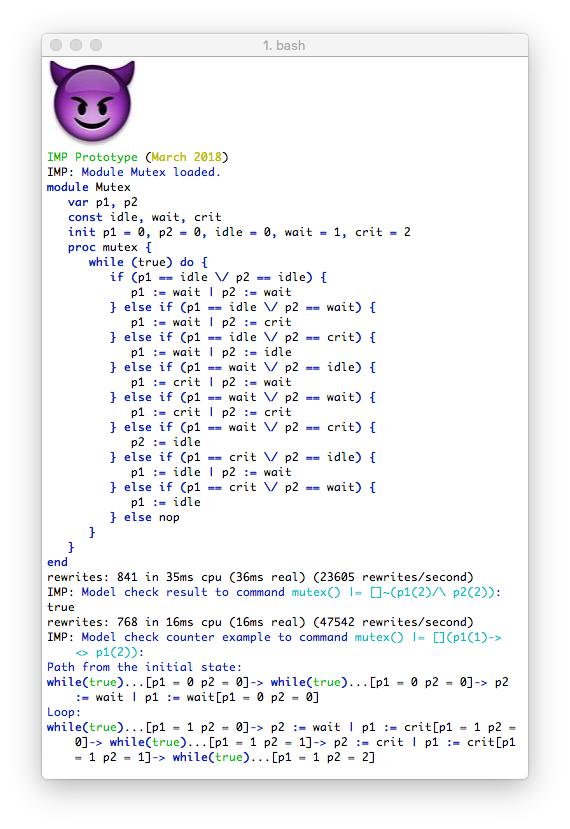
\includegraphics[width=\columnwidth]{imp-mutex.png} \end{center}
\caption{Model checking a Mutex protocol in \textsc{Imp} that is safe but not live.}
\label{fig:imp-mutex}
\end{figure}

% Descent functions

% Read-eval-loop

% Parsing

% Transforming

% Executing a command

% Pretty-printing

\paragraph{\textsc{Imp}'s command-line interface}

In Listing~\ref{lst:imp-cli} we describe an excerpt of the implementation for \textsc{Imp}'s command-line interface, detailing only the module inclusions, sort declarations for the command-line state and rules for loading an \textsc{Imp} program. A full description is not possible due to space constraints. However, the pattern explained in this excerpt is the same for every command: a qidlist denotes the input, a different meta-function is called on them, depending on the input, that updates or not the state of IMP's command-line interface and or the output of the system as whole, with a message to the end user.  

First, module IMP-INTERFACE includes LOOP-MODE module.
Module LOOP-MODE declares operation \texttt{op [\_,\_,\_] : QidList State QidList -> System} that declares the state of the loop-mode instance, in our case, \textsc{Imp} loop mode. IMP-INTERFACE than renames LOOP-MODE' sort State to LoopState, to avoid a name clash. Next, modules COMPILE-IMP-TO-$\uppi$-lib and IMP-PRETTY-PRINTING are included, responsible for the functionalities that their names stand for. 
Operation \texttt{op <\_;\_;\_> : MetaIMPModule Dec? QidList -> IMPState} represents the state of the command-line interface, which is a triple comprised by (i) the meta-representation of an \textsc{Imp} module, (ii) the $\uppi$-lib representation of the \textsc{Imp} module in the first projection, and (iii) a qid list denoting the message from the last processed command. Rule labeled \texttt{in} is responsible for processing the input of an \textsc{Imp} module, therefore, in this case, the first projection of the System term contains a list of qids representing an \textsc{Imp} module. Should the parsing process be successful, variable \texttt{T:ResultPair?} will be bound to a pair whose first projection is the term resulting from  parsing and in the second projection its sort, or a unary function, of sort \texttt{ResultPair?}, denoting that the parsing process was not properly carried on, with a parameter representing the qid where the parsing process failed. With a successful parsing, the following term becomes now the state of the system
\begin{maude}
< getTerm(T:ResultPair?) ; compileMod(getTerm(T:ResultPair?)) ; 
   'IMP: '\b 'Module Q:Qid 'loaded. '\o  >
\end{maude}
where \texttt{getTerm(T:ResultPair?)} denotes the meta-term, according to \textsc{Imp}'s grammar, representing the input module, \texttt{compileMod(getTerm(T:ResultPair?))} denotes the input module in $\uppi$-lib, in the second projection, and the third component of the \texttt{IMPState} triple is a qidlist represents a message to the user know informing that the module was properly loaded.

\begin{maude}[caption=\textsc{Imp}'s command-line interface in Maude, label=lst:imp-cli]
mod IMP-INTERFACE is
 pr LOOP-MODE * (sort State to LoopState).
 pr COMPILE-IMP-TO-$\uppi$-lib .
 pr IMP-PRETTY-PRINTING .

 sorts Dec? MetaIMPModule Command IMPState .
 subsort Term < MetaIMPModule .
 subsort Dec < Dec? .
 subsort IMPState < LoopState .

 op noDec : -> Dec? .
 op noModule : -> MetaIMPModule .
 op idle : -> Command .
 op <_;_;_> : MetaIMPModule Dec? QidList -> IMPState .

 $\ldots$
 vars QIL QIL' QIL'' QIL1 QIL2 : QidList .

 *** Loading a module.
 crl [in] : ['module Q:Qid QIL, < M:MetaIMPModule ; D:Dec? ; QIL' >, QIL''] =>
             if (T:ResultPair? :: ResultPair)
             then 
                 [nil, < getTerm(T:ResultPair?) ; 
                           compileMod(getTerm(T:ResultPair?)) ; 
                           'IMP: '\b 'Module Q:Qid 'loaded. '\o  >, QIL'']
             else [nil, < noModule ; noDec ; nil >, 
                      printParseError('module Q:Qid QIL, T:ResultPair?)]
             fi
 if T:ResultPair? :=
    metaParse(upModule('IMP-GRAMMAR, false), 
      'module Q:Qid QIL, 'ModuleDecl) .

 *** Viewing a module.
 crl [view] : ['view , < M:MetaIMPModule ; D:Dec ; QIL' >, QIL''] =>
                  [nil, < M:MetaIMPModule ; D:Dec ; QIL' >,
                           printModule(M:MetaIMPModule)]
 if M:MetaIMPModule =/= noModule .

 $\ldots$
endm
\end{maude}

\paragraph{\textsc{Imp} parser}

To write a parser in Maude one has to first define the grammar of the language as a Maude functional module. The IMP-GRAMMAR module is the first argument in the function call to metaParse in Rule \texttt{in} of module IMP-INTERFACE in Listing~\ref{lst:imp-cli}.
Essentially, variables (or non-terminals) are represented by sorts, terminals by constants and grammar rules are represented by operations. Listing~\ref{lst:imp-grammar} encodes an excerpt of the \textsc{Imp} grammar, only enough to discuss the main elements of the grammar representation: we exemplify it with sum expressions
%, two commands and two declarations. 
Sort ExpressionDecl, for instance, specifies both arithmetic and Boolean expressions. A grammar rule relating two grammar variables is represented by a subsort declaration. Therefore, PredicateDecl, the sort for Boolean expressions, is a subsort of ExpressionDecl.   

\begin{maude}[caption=\textsc{Imp} grammar as a Maude functional module, label=lst:imp-grammar]
fmod IMP-GRAMMAR is
 pr TOKEN . pr RAT .
 inc PREDICATE-DECL . inc COMMAND-DECL .
 sorts VariablesDecl ConstantsDecl OperationsDecl ProcDeclList
       ProcDecl FormalsDecl BlockCommandDecl ExpressionDecl
       InitDecl InitDeclList InitDecls ClausesDecl
       ModuleDecl Expression .

 subsort InitDecl < InitDeclList .
 subsort VariablesDecl ConstantsDecl ProcDeclList InitDecls < ClausesDecl .
 subsort BlockCommandDecl < CommandDecl .
 subsort ProcDecl < ProcDeclList .
 subsort PredicateDecl < ExpressionDecl .

$\ldots$

 *** Arithmetic expressions
 op _+_ : Token Token -> ExpressionDecl [gather(e E) prec 15] .
 op _+_ : Token ExpressionDecl -> ExpressionDecl [gather(e E) prec 15] .
 op _+_ : ExpressionDecl Token -> ExpressionDecl [gather(e E) prec 15] .
 op _+_ : ExpressionDecl ExpressionDecl -> ExpressionDecl [gather(e E) prec 15] .

$\ldots$
endfm
\end{maude}
 
The \texttt{prec} operator attribute declares the precedence of the operator, as commonly available in parser generators. A precedence value associates an Integer greater than $0$ to terms with the given operator at the top. The gather attribute allows for the specification of precedence constraints among the operands and an operator. For instance, the pattern \texttt{gather(e, E)} specifies that the first operand must have strictly lower precedence than the given operator, while the second operand must have a lower or equal precedence with respect to the given operator. 

\paragraph{\textsc{Imp} to $\uppi$-lib transformer}

Compilation from IMP to $\uppi$-lib is quite trivial as there exists a one-to-one correspondence between IMP constructions and $\uppi$-lib. Essentially, an IMP {\Tt{}module\nwendquote} gives rise to a $\uppi$-lib {\Tt{}dec\nwendquote}. IMP {\Tt{}var\nwendquote} and {\Tt{}const\nwendquote} are declarations and so is a {\Tt{}proc\nwendquote} declaration that gives rise to a {\Tt{}prc\nwendquote} declaration in $\uppi$-lib. 
\begin{maude}
mod COMPILE-IMP-TO-$\uppi$-lib is
 inc PREDICATE-DECL .
 inc COMMAND-DECL .
 pr $\uppi$-lib .
 pr META-LEVEL .

$\ldots$
\end{maude}

The compilation from IMP to $\uppi$-lib exp relates IMP tokens to $\uppi$-lib Id, IMP arithmetic and boolean expressions to $\uppi$-lib Exp. In particular, the compilation of a {\Tt{}token\nwendquote} has to check if the token is a primitive type, either {\Tt{}Rat\nwendquote} (for Rational numbers) or {\Tt{}Bool\nwendquote} (for Boolean values), or an identifier. Since {\Tt{}Rat\nwendquote} and {\Tt{}Bool\nwendquote} are tokenized and we need Maude metalevel descent function {\Tt{}downTerm\nwendquote} to help us parse them into proper constants
 
\begin{maude}
 op compileId : Qid -> Id .
 eq compileId(I:Qid) = idn(downTerm(I:Qid, 'Qid)) .

 op compileId : Term -> Id .
 eq compileId('token[I:Qid]) =
    if (metaParse(upModule('RAT, false), 
         downTerm(I:Qid, 'Qid), 'Rat)  :: ResultPair)
        then rat(downTerm(getTerm(metaParse(upModule('RAT, false),
              downTerm(I:Qid, 'Qid), 'Rat)), 1/2))
    else
     if (metaParse(upModule('BOOL, false), 
          downTerm(I:Qid, 'Qid), 'Bool) :: ResultPair)
     then boo(downTerm(getTerm(metaParse(upModule('BOOL, false),
                   downTerm(I:Qid, 'Qid), 'Bool)), true))
     else idn(downTerm(I:Qid, 'Qid))
     fi
    fi .
\end{maude}

Arithmetic expressions are mapped to their prefixed counterpart in $\uppi$-lib, e.g, an IMP expression {\Tt{}a\ +\ b\nwendquote} is compiled to {\Tt{}add(compileExp(a),\ compileExp(b))\nwendquote}.
\begin{maude}
 op compileExp : Term -> Exp .
 ceq compileExp(I:Qid) = compileId(I:Qid) 
  if not(I:Qid :: Constant) .
 eq compileExp('token[I:Qid]) = compileId('token[I:Qid]) .
 eq compileExp('_+_[T1:Term, T2:Term]) =
     add(compileExp(T1:Term), compileExp(T2:Term)) .
 eq compileExp('_-_[T1:Term, T2:Term]) =
     sub(compileExp(T1:Term), compileExp(T2:Term)) .
 eq compileExp('_*_[T1:Term, T2:Term]) =
     mul(compileExp(T1:Term), compileExp(T2:Term)) .
 eq compileExp('_/_[T1:Term, T2:Term]) =
     div(compileExp(T1:Term), compileExp(T2:Term)) .
\end{maude}

%\paragraph{Pretty-printers}
% 
% \begin{maude}
% mod IMP-PRETTY-PRINTING is
% pr $\uppi$-lib-MODEL-CHECKER .
% pr COMPILE-TO-PYTHON . 
% pr INT .
%
%  *** Pretty-printing IMP Declarations
% op printModule : Term -> QidList .
% eq printModule('module__end[T1:Term, T2:Term]) =
%    printToken('module) printTokens(T1:Term)
%       printClauses(T2:Term)
%       '\n printToken('end) .
% \end{maude}


\section{The complete $\uppi$-lib code in Maude}

\nwfilename{../bplc.noweb}\nwbegincode{1}\moddef{gsmc}\endmoddef\nwstartdeflinemarkup\nwenddeflinemarkup
fmod VALUE-SORT is
    sort Value . 
endfm

fmod CONTROL-SORT is
    sort Control . 
endfm

view Control from TRIV to CONTROL-SORT is
    sort Elt to Control . 
endv

view Value from TRIV to VALUE-SORT is
    sort Elt to Value . 
endv

--- Note: AI theories are not currently supported by Maude unification, 
--- as of Alpha 115. 
fmod GNELIST\{X :: TRIV\} is
    pr NAT .
    sorts GNeList\{X\} .
    subsort X$Elt < GNeList\{X\} .

    op __ : GNeList\{X\} GNeList\{X\} -> GNeList\{X\} [ctor assoc prec 25] . 
endfm

--------------------------------------------------------------
--- GSMC semantics for basic programming language constructs .

fmod VALUE-STACK is
    pr GNELIST\{Value\} * (sort GNeList\{Value\} to NeValueStack) .
    sort ValueStack .
    subsort NeValueStack < ValueStack .
    op evs : -> ValueStack . 
    op __ : ValueStack ValueStack -> ValueStack [ditto] .       
endfm

fmod CONTROL-STACK is
    pr GNELIST\{Control\} * (sort GNeList\{Control\} to NeControlStack) .
    sort ControlStack .
    subsort NeControlStack < ControlStack .
    op ecs : -> ControlStack . 
    op __ : ControlStack ControlStack -> ControlStack [ditto] .         
endfm

fmod MEMORY-SORTS is
    sorts Loc Storable . 
endfm

view Loc from TRIV to MEMORY-SORTS is
    sort Elt to Loc . 
endv

view Storable from TRIV to MEMORY-SORTS is
    sort Elt to Storable . 
endv

fmod MEMORY is
    pr NAT .
    ex MAP\{Loc,Storable\} * (sort Entry\{Loc,Storable\} to Cell,
       sort Map\{Loc,Storable\} to Store,
       op undefined to undefloc, op empty to noStore).
    ex SET\{Loc\} * (op empty to noLocs) .

    op loc : Nat -> Loc [ctor] .
    op newLoc : Store -> Loc .
    op $newLoc : Store Nat -> Loc .
    eq newLoc(noStore) = loc(0) .
    ceq newLoc(S:Store) = $newLoc(S:Store, 0) if S:Store =/= noStore .
    eq $newLoc(noStore, N:Nat) = loc(N:Nat + 1) .
    ceq $newLoc((S:Store, loc(N:Nat) |-> O:Storable), N':Nat) =
        $newLoc(S:Store, N:Nat) if N:Nat >= N':Nat .
    ceq $newLoc((S:Store, loc(N:Nat) |-> O:Storable), N':Nat) =
        $newLoc(S:Store, N':Nat) if N:Nat < N':Nat .

    op $free : Loc Store -> Store .
    eq $free(L:Loc, ((L:Loc |-> O:Storable), S:Store)) = S:Store .
    eq $free(L:Loc, S:Store) = S:Store [owise] .

    op free : Set\{Loc\} Store -> Store .
    eq free(noLocs, S:Store) = S:Store .
    eq free((L:Loc , SL:Set\{Loc\}), S:Store) =
       free(SL:Set\{Loc\}, $free(L:Loc, S:Store)) [owise] . 
endfm

fmod ENV-SORTS is
    sorts Id Bindable . 
endfm

view Id from TRIV to ENV-SORTS is sort Elt to Id . endv

view Bindable from TRIV to ENV-SORTS is sort Elt to Bindable . endv

fmod ENV is
    ex MAP\{Id,Bindable\} * (sort Entry\{Id,Bindable\} to Bind,
       sort Map\{Id,Bindable\} to Env,
       op undefined to undefid, op empty to noEnv). 
endfm

-----------------------------
--- Generalized SMC machines.

fmod SEMANTIC-COMPONENTS is
    sorts SemComp . 
endfm

view SemComp from TRIV to SEMANTIC-COMPONENTS is
    sort Elt to SemComp . 
endv

fmod GSMC is
    ex VALUE-STACK .
    ex MEMORY .
    ex CONTROL-STACK .
    ex ENV . 
    ex SET\{SemComp\} * (op empty to noSemComp) .

    sorts Attrib Conf EnvAttrib StoreAttrib ControlAttrib ValueAttrib .
    subsort EnvAttrib StoreAttrib ControlAttrib ValueAttrib < Attrib  .
    op <_> : Set\{SemComp\} -> Conf [format(c! c! c! o)] . 

    --- Semantic components
    op env : -> EnvAttrib .
    op sto : -> StoreAttrib .
    op cnt : -> ControlAttrib .
    op val : -> ValueAttrib .
    op _:_ : EnvAttrib Env -> SemComp [ctor format(c! b! o o)] .
    op _:_ : StoreAttrib Store -> SemComp [ctor format(r! b! o o)] .
    op _:_ : ControlAttrib ControlStack -> SemComp [ctor format(c! b! o o)] .
    op _:_ : ValueAttrib ValueStack -> SemComp [ctor format(c! b! o o)] .
endfm
\nwendcode{}\nwbegindocs{2}\nwdocspar

\section{Basic Programming Languages Constructs}

\begin{itemize}

\item Expressions: identifier, rational numbers, Boolean values,
arithmetic and predicates. Semantic components: Identifiers require
the environment and the store. The remaining constructs do not require
any semantic component.

\item Commands: print, assignment, sequence, choice, block,
conditional, and loop. Print updates output. The remaining constructs
affect only the store.

\item Declarations: variables, constants, and procedures. These
constructs affect the environment.

\item Abnormal termination: exit. Command exit changes the semantic
component that indicates abnormal termination. The behavior of command
composition is also affected by this semantic component.

\end{itemize}

\subsection{Expressions}
\nwenddocs{}\nwbegincode{3}\moddef{bplc-exp}\endmoddef\nwstartdeflinemarkup\nwenddeflinemarkup
fmod EXP is
    pr QID .
    pr RAT .
    pr GSMC .  

    sorts Exp BExp AExp .
    subsort Id < BExp AExp < Exp < Control .

    --- Identifiers
    op idn : Qid -> Id [ctor format(!g o)] .
    
    --- Arithmetic
    op rat : Rat -> AExp [ctor format(!g o)] .
    op add : AExp AExp -> AExp [format(! o)] .
    op sub : AExp AExp -> AExp [format(! o)] .
    op mul : AExp AExp -> AExp [format(! o)] .
    op div : AExp AExp -> AExp [format(! o)] .

    ops ADD SUB MUL DIV : -> Control [ctor] .

    --- Boolean expressions
    op boo : Bool -> AExp [ctor format(!g o)] .
    op gt : Exp Exp -> BExp [format(! o)] .
    op ge : Exp Exp -> BExp [format(! o)] .
    op lt : Exp Exp -> BExp [format(! o)] .
    op le : Exp Exp -> BExp [format(! o)] .
    op eq : Exp Exp -> BExp [format(! o)] .
    op neg : BExp -> BExp [format(! o)] .
    op and : BExp BExp -> BExp [format(! o)] .
    op or : BExp BExp -> BExp [format(! o)] .

    ops LT LE EQ NEG AND OR : -> Control [ctor] .

    op store : Rat -> Storable [ctor format(ru! o)] .
    op store : Bool -> Storable [ctor format(ru! o)] .
    op bind : Loc -> Bindable [ctor] .
    op bind : Rat -> Bindable [ctor] .
    op bind : Bool -> Bindable [ctor] .

    op val : Storable -> Value [ctor] .
    op val : Rat -> Value [ctor] .
    op val : Bool -> Value [ctor] .
    op val : Loc -> Value [ctor] .
    op val : Id -> Value [ctor] .

    var ... : Set\{SemComp\} .

    eq gt(E1:Exp, E2:Exp) = neg(le(E1:Exp, E2:Exp)) .
    eq ge(E1:Exp, E2:Exp) = neg(lt(E1:Exp, E2:Exp)) .

    eq [rat-exp] :
        < cnt : (rat(R:Rat) C:ControlStack), val : SK:ValueStack, ... > 
     =
        < cnt : C:ControlStack,
          val : (val(R:Rat) SK:ValueStack), ... > [variant] .

    eq [bool-exp] :
        < cnt : (boo(B:Bool) C:ControlStack), val : SK:ValueStack, ... > 
     =
        < cnt : C:ControlStack,
          val : (val(B:Bool) SK:ValueStack), ... > [variant] .

    eq [add-exp] :
        < cnt : (add(E1:Exp, E2:Exp) C:ControlStack), ... > 
     =
        < cnt : (E1:Exp E2:Exp ADD C:ControlStack), ... > [variant] .

    eq [add-exp] :
        < cnt : (ADD C:ControlStack),
          val : (val(R1:Rat) val(R2:Rat) SK:ValueStack), ... > 
     =
        < cnt : C:ControlStack,
          val : (val(R1:Rat + R2:Rat) SK:ValueStack), ... > [variant] .

    eq [sub-exp] :
        < cnt : (sub(E1:Exp, E2:Exp) C:ControlStack), ... > 
     =
        < cnt : (E1:Exp E2:Exp SUB C:ControlStack), ... > [variant] .

    eq [sub-exp] :
        < cnt : (SUB C:ControlStack),
          val : (val(R1:Rat) val(R2:Rat) SK:ValueStack), ... > 
     =
        < cnt : C:ControlStack,
          val : (val(R2:Rat - R1:Rat) SK:ValueStack), ... > [variant] .

    eq [mul-exp] :
        < cnt : (mul(E1:Exp, E2:Exp) C:ControlStack), ... > 
     =
        < cnt : (E1:Exp E2:Exp MUL C:ControlStack), ... > [variant] .

    eq [mul-exp] :
        < cnt : (MUL C:ControlStack),
          val : (val(R1:Rat) val(R2:Rat) SK:ValueStack), ... > 
     =
        < cnt : C:ControlStack,
          val : (val(R1:Rat * R2:Rat) SK:ValueStack), ... > [variant] .

    eq [div-exp] :
        < cnt : (div(E1:Exp, E2:Exp) C:ControlStack), ... > 
     =
        < cnt : (E1:Exp E2:Exp DIV C:ControlStack), ... > [variant] .

    eq [div-exp] :
        < cnt : (DIV C:ControlStack),
          val : (val(R1:Rat) val(R2:NzRat) SK:ValueStack), ... > 
     =
        < cnt : C:ControlStack,
          val : (val(R1:Rat / R2:NzRat) SK:ValueStack), ... > [variant] .

    eq [lt-exp] :
        < cnt : (lt(E1:Exp, E2:Exp) C:ControlStack), ... > 
     =
        < cnt : (E2:Exp E1:Exp LT C:ControlStack), ... > [variant] .

    eq [lt-exp] :
        < cnt : (LT C:ControlStack),
          val : (val(R1:Rat) val(R2:Rat) SK:ValueStack), ... > 
     =
        < cnt : C:ControlStack,
          val : (val(R1:Rat < R2:Rat) SK:ValueStack), ... > [variant] .

    eq [le-exp] :
        < cnt : (le(E1:Exp, E2:Exp) C:ControlStack), ... > 
     =
        < cnt : (E2:Exp E1:Exp LE C:ControlStack), ... > [variant] .

    eq [le-exp] :
        < cnt : (LE C:ControlStack),
          val : (val(R1:Rat) val(R2:Rat) SK:ValueStack), ... > 
     =
        < cnt : C:ControlStack,
          val : (val(R1:Rat <= R2:Rat) SK:ValueStack), ... > [variant] .

    eq [eq-exp] :
        < cnt : (eq(E1:Exp, E2:Exp) C:ControlStack), ... > 
     =
        < cnt : (E2:Exp E1:Exp EQ C:ControlStack), ... > [variant] .

    eq [eq-exp] :
        < cnt : (EQ C:ControlStack),
          val : (val(R1:Rat) val(R2:Rat) SK:ValueStack), ... > 
     =
        < cnt : C:ControlStack,
          val : (val(R1:Rat == R2:Rat) SK:ValueStack), ... > [variant] .

    eq [eq-exp] :
        < cnt : (EQ C:ControlStack),
          val : (val(B1:Bool) val(B2:Bool) SK:ValueStack), ... > 
     =
        < cnt : C:ControlStack,
          val : (val(B1:Bool == B2:Bool) SK:ValueStack), ... > [variant] .

    eq [neg-exp] :
        < cnt : (neg(E:Exp) C:ControlStack), ... > 
     =
        < cnt : (E:Exp NEG C:ControlStack), ... > [variant] .

    eq [neg-exp] :
        < cnt : (NEG C:ControlStack),
          val : (val(B:Bool) SK:ValueStack), ... > 
     =
        < cnt : C:ControlStack,
          val : (val(not(B:Bool)) SK:ValueStack), ... > [variant] .

    eq [and-exp] :
        < cnt : (and(E1:Exp, E2:Exp) C:ControlStack), ... > 
     =
        < cnt : (E1:Exp E2:Exp AND C:ControlStack), ... > [variant] .

    eq [and-exp] :
        < cnt : (AND C:ControlStack),
          val : (val(B1:Bool) val(B2:Bool) SK:ValueStack), ... > 
     =
        < cnt : C:ControlStack,
          val : (val(B1:Bool and B2:Bool) SK:ValueStack), ... > [variant] .

    eq [or-exp] :
        < cnt : (or(E1:Exp, E2:Exp) C:ControlStack), ... > 
     =
        < cnt : (E1:Exp E2:Exp OR C:ControlStack), ... > [variant] .

    eq [and-exp] :
        < cnt : (OR C:ControlStack),
          val : (val(B1:Bool) val(B2:Bool) SK:ValueStack), ... > 
     =
        < cnt : C:ControlStack,
          val : (val(B1:Bool or B2:Bool) SK:ValueStack), ... > [variant] .

    eq [variable-exp] :
        < env : (I:Id |-> bind(L:Loc), E:Env),
          sto : (L:Loc |-> store(R:Rat), S:Store),
          cnt : (I:Id C:ControlStack), val : SK:ValueStack, ... > 
     =
        < env : (I:Id |-> bind(L:Loc), E:Env),
          sto : (L:Loc |-> store(R:Rat), S:Store),
          cnt : C:ControlStack ,
          val : (val(R:Rat) SK:ValueStack) , ... > [variant] .

    eq [variable-exp] :
        < env : (I:Id |-> bind(L:Loc), E:Env),
          sto : (L:Loc |-> store(B:Bool), S:Store),
          cnt : (I:Id C:ControlStack), val : SK:ValueStack, ... > 
     =
        < env : (I:Id |-> bind(L:Loc), E:Env),
          sto : (L:Loc |-> store(B:Bool), S:Store),
          cnt : C:ControlStack ,
          val : (val(B:Bool) SK:ValueStack) , ... > [variant] .

    eq [constant-rat-exp] :
        < env : (I:Id |-> bind(R:Rat), E:Env), cnt : (I:Id C:ControlStack),
          val : SK:ValueStack , ... > 
     =
        < env : (I:Id |-> bind(R:Rat), E:Env), cnt : C:ControlStack,
          val : (val(R:Rat) SK:ValueStack), ... > [variant] .

    eq [constant-bool-exp] :
        < env : (I:Id |-> bind(B:Bool), E:Env), cnt : (I:Id C:ControlStack),
          val : SK:ValueStack, ... > 
     =
        < env : (I:Id |-> bind(B:Bool), E:Env), cnt : C:ControlStack,
          val : (val(B:Bool) SK:ValueStack), ... > [variant] .        
endfm
\nwendcode{}\nwbegindocs{4}\nwdocspar

\subsection{Commands}
\nwenddocs{}\nwbegincode{5}\moddef{bplc-cmd}\endmoddef\nwstartdeflinemarkup\nwenddeflinemarkup
mod CMD is
    pr EXP .

    sort Cmd .
    subsort Cmd < Control .

    op nop : -> Cmd [ctor format(! o)] .
    op choice : Cmd Cmd -> Cmd [ctor assoc comm format(! o)] .
    op assign : Id Exp -> Cmd [ctor format(! o)] .
    op loop : Exp Cmd -> Cmd [ctor format(! o)] .
    op if : Exp Cmd Cmd -> Cmd [ctor format(! o)] .

    ops ASSIGN LOOP IF : -> Control [ctor] . 

    op val : Cmd -> Value [ctor] .
    
    var ... : Set\{SemComp\} . var E : Env . var S : Store .
    var C : ControlStack . var V : ValueStack .

    eq [nop-cmd] :
        < cnt : nop C, ... > = < cnt : C, ... > [variant] .

    rl [choice-cmd] :
        < cnt : choice(M1:Cmd, M2:Cmd) C, ... > =>
        < cnt : M1:Cmd C, ... > . --- [narrowing] .

    eq [assign-cmd] :
        < env : (I:Id |-> bind(L:Loc), E),
          cnt : (assign(I:Id, E:Exp) C),
          val : V, ... > 
     =
        < env : (I:Id |-> bind(L:Loc), E),
          cnt : (E:Exp ASSIGN C),
          val : (val(I:Id) V), ... > [variant] .

    eq [assign-cmd] :
        < env : (I:Id |-> bind(L:Loc), E),
          sto : (L:Loc |-> T:Storable, S),
          cnt : (ASSIGN C),
          val : (val(R:Rat) val(I:Id) V), ... > 
     =
        < env : (I:Id |-> bind(L:Loc), E),
          sto : (L:Loc |-> store(R:Rat), S),
          cnt : C,
          val : V, ... > [variant] .

    eq [assign-cmd] :
        < env : (I:Id |-> bind(L:Loc), E),
          sto : (L:Loc |-> T:Storable, S),
          cnt : (ASSIGN C),
          val : (val(B:Bool) val(I:Id) V), ... > 
     =
        < env : (I:Id |-> bind(L:Loc), E),
          sto : (L:Loc |-> store(B:Bool), S),
          cnt : C,
          val : V, ... > [variant] .

    eq [loop] :
        < cnt : loop(E:Exp, K:Cmd) C, val : V, ... > 
     =
        < cnt : E:Exp LOOP C,
          val : val(loop(E:Exp, K:Cmd)) V, ... > [variant] .

    rl [loop] :
        < cnt : LOOP C,
          val : val(true) val(loop(E:Exp, K:Cmd)) V, ... > 
    =>
        < cnt : K:Cmd loop(E:Exp, K:Cmd) C,
          val : V, ... > . --- [narrowing] .

    eq [loop] :
        < cnt : LOOP C,
          val : val(false) val(loop(E:Exp, K:Cmd)) V, ... > 
     =
        < cnt : C, val : V, ... > [variant] .

    eq [if] :
       < cnt : if(E:Exp, K1:Cmd, K2:Cmd) C, val : V, ... > 
     =
       < cnt : E:Exp IF C,
         val : val(if(E:Exp, K1:Cmd, K2:Cmd)) V, ... > [variant] .

    eq [if] :
       < cnt : IF C,
         val : val(true) val(if(E:Exp, K1:Cmd, K2:Cmd)) V, ... > 
     =
       < cnt : K1:Cmd C,
         val : V, ... > [variant] .

    eq [if] :
       < cnt : IF C,
         val : val(false) val(if(E:Exp, K1:Cmd, K2:Cmd)) V, ... > 
     =
       < cnt : K2:Cmd C,
         val : V, ... > [variant] .
endm
\nwendcode{}\nwbegindocs{6}\nwdocspar

\subsection{Declarations}
\nwenddocs{}\nwbegincode{7}\moddef{bplc-dec}\endmoddef\nwstartdeflinemarkup\nwenddeflinemarkup
mod DEC is
    ex CMD .

    sorts Abs Blk Dec Formal Formals Actual Actuals LocsAttrib .
    subsort Actuals Dec < Control .
    subsort Formal < Formals .
    subsort Exp < Actual < Actuals .
    subsort Blk < Cmd .
    subsort Abs < Bindable .

    op cns : Id Exp -> Dec [ctor format(! o)] .
    op ref : Id Exp -> Dec [ctor format(! o)] .
    op prc : Id Blk -> Dec [ctor format(! o)] .
    op prc : Id Formals Blk -> Dec [ctor format(! o)] .
    op par : Id -> Formal [ctor format(! o)] .
    op vod : -> Formal [ctor format(! o)] .
    op for : Formals Formals -> Formals [ctor assoc format(! o)] .
    op dec : Dec Dec -> Dec [ctor format(! o)] .
    op blk : Cmd -> Blk [ctor format(! o)] .
    op blk : Dec Cmd -> Blk [ctor format(! o)] .
    op cal : Id -> Cmd [ctor format(! o)] .
    op cal : Id Actuals -> Cmd [ctor format(! o)] .
    op act : Actuals Actuals -> Actuals [ctor assoc format(! o)] .
    ops CNS REF CAL BLK FRE : -> Control [ctor] .

    op val : Env -> Value [ctor] .
    op val : Loc -> Value [ctor] .
    op val : Abs -> Value [ctor] .
    op val : Set\{Loc\} -> Value [ctor] .
    
    op abs : Blk -> Abs [ctor] .
    op abs : Formals Blk -> Abs [ctor] .
    op locs : -> LocsAttrib [ctor] .
    op _:_ : LocsAttrib Set\{Loc\} -> SemComp [ctor format(c! b! o o)] .

    var ... : Set\{SemComp\} . vars E E' : Env . var S : Store .
    var C : ControlStack . var V : ValueStack .

    eq [blk] :
        < cnt : blk(D:Dec, M:Cmd) C, env : E , val : V , locs : SL:Set\{Loc\} , ... > 
     =
        < cnt : D:Dec M:Cmd BLK C, env : E , 
                  val : val(E) val(SL:Set\{Loc\}) V , 
                  locs : noLocs , ... > [variant] .

    eq [blk] :
        < cnt : blk(M:Cmd) C, env : E , val : V , locs : SL:Set\{Loc\} , ... > 
     =
        < cnt : M:Cmd BLK C, env : E , 
                  val : val(E) val(SL:Set\{Loc\}) V , 
                  locs : noLocs , ... > [variant] .

    eq [blk] :
        < cnt : BLK C ,
          env : E' ,
          val : val(E) val(SL:Set\{Loc\}) V ,
         locs : SL':Set\{Loc\},
          sto : S:Store, ... > 
     =
        < cnt : C ,
          env : E ,
          val : V ,
         locs : SL:Set\{Loc\},
          sto : free(SL':Set\{Loc\}, S:Store), ... > [variant] .

    eq [ref] :
        < cnt : ref(I:Id, X:Exp) C , val : V , ... > =
        < cnt : X:Exp REF C , val : val(I:Id) V , ... > [variant] .

    eq [ref] :
        < cnt : REF C, env : E ,
          sto : S ,
          val : val(R:Rat) val(I:Id) V ,
          locs : SL:Set\{Loc\} , ... > 
     =
        < cnt : C ,
          env : insert(I:Id, bind(newLoc(S)), E) ,
          sto : insert(newLoc(S), store(R:Rat), S) ,
          val : V ,
          locs : (newLoc(S) , SL:Set\{Loc\}) , ... > [variant] .

    eq [cns] :
        < cnt : cns(I:Id, X:Exp) C , val : V , ... > =
        < cnt : X:Exp CNS C , val : val(I:Id) V , ... > [variant] .

    eq [cns] :
        < cnt : CNS C, env : E , val : val(R:Rat) val(I:Id) V , ... > =
        < cnt : C ,
          env : (I:Id |-> bind(R:Rat) , E) ,
          val : V , ... > [variant] .

    eq [prc] :
        < cnt : prc(I:Id, F:Formals, B:Blk) C, env : E, ... > =
        < cnt : C,
          env : insert(I:Id, abs(F:Formals, B:Blk), E), ... > [variant] .

    eq [prc] :
        < cnt : prc(I:Id, B:Blk) C, env : E, ... > =
        < cnt : C,
          env : insert(I:Id, abs(B:Blk), E), ... > [variant] .

    eq [dec] :
        < cnt : dec(D1:Dec, D2:Dec) C, ... > =
        < cnt : D1:Dec D2:Dec C , ... > [variant] .

    eq [cal] :
        < cnt : cal(I:Id) C, ... > =
        < cnt : I:Id CAL C, ... > [variant] .

    eq [cal] :
        < cnt : cal(I:Id, A:Actuals) C, ... > =
        < cnt : I:Id A:Actuals CAL C, ... > [variant] .

    eq [cal] :
        < cnt : CAL C,
          val : V1:ValueStack
          val(abs(F:Formals, B:Blk)) V2:ValueStack, ... > =
        < cnt : addDec(match(F:Formals, V1:ValueStack), B:Blk) C,
          val : V2:ValueStack, ... > [variant] .

    eq [cal] :
        < cnt : CAL C,
          val : val(abs(B:Blk)) V:ValueStack, ... > =
        < cnt : B:Blk C,
          val : V:ValueStack, ... > [variant] .

    eq [prc-id] :
        < cnt : (I:Id C),
          env : (I:Id |-> A:Abs, E),
          val : V , ... > =
        < cnt : C,
          env : (I:Id |-> A:Abs, E),
          val : (val(A:Abs) V), ... > [variant] .

    eq [act] :
        < cnt : act(E:Exp, A:Actuals) C, ... > =
        < cnt : A:Actuals E:Exp C, ... > [variant] .

    op match : Formals ValueStack -> Dec .
    eq match(par(I:Id), val(R:Rat)) = ref(I:Id, rat(R:Rat)) .
    eq match(par(I:Id), val(B:Bool)) = ref(I:Id, boo(B:Bool)) .
    eq match(for(F:Formal, L:Formals), (V:Value VS:ValueStack)) =
        dec(match(F:Formal, V:Value),
          match(L:Formals, VS:ValueStack)) .

    op addDec : Dec Blk -> Blk .
    eq addDec(D:Dec, B:Blk) = blk(D:Dec, B:Blk) .
endm
\nwendcode{}\nwbegindocs{8}\nwdocspar

\subsection{Output}
\nwenddocs{}\nwbegincode{9}\moddef{bplc-out}\endmoddef\nwstartdeflinemarkup\nwenddeflinemarkup
mod OUT is
    ex DEC .

    sort OutAttrib .

    op out : -> OutAttrib [ctor] .
    op _:_ : OutAttrib ValueStack -> SemComp [ctor format(c! b! o o)] .
    op print : Exp -> Cmd [ctor format(! o)] .
    op PRINT : -> Control [ctor] .

    var ... : Set\{SemComp\} .

    op out : Conf -> NeValueStack [ctor] .
    eq out(< out : V:NeValueStack , ... >) = V:NeValueStack .

    eq [print] :
        < cnt : (print(E:Exp) C:ControlStack), ... > =
        < cnt : (E:Exp PRINT C:ControlStack), ... > [variant] .

    eq [print] :
        < cnt : (PRINT C:ControlStack),
          val : val(R:Rat) V:ValueStack,
          out : O:ValueStack, ... > =
        < cnt : C:ControlStack,
          val : V:ValueStack,
          out : val(R:Rat) O:ValueStack , ... > [variant] .
endm
\nwendcode{}\nwbegindocs{10}\nwdocspar

\subsection{Abnormal termination}
\nwenddocs{}\nwbegincode{11}\moddef{bplc-ext}\endmoddef\nwstartdeflinemarkup\nwenddeflinemarkup
mod COMMAND-SEQ-AND-ABNORMAL-TERMINATION is
    ex OUT .

    sorts ExcAttrib Exc .
    
    --- Sequences had to be moved "down" from CMD to this module because
    --- the evaluation of the next command only takes place if no
    --- exit was executed.
    op seq : Cmd Cmd -> Cmd [format(! o)] .

    op exit : Exp -> Cmd [format(! o)] .
    op EXT : -> Exc .
    op EXIT : -> Control .
    op CNT : -> Exc .
    op exc : -> ExcAttrib .
    op _:_ : ExcAttrib Exc -> SemComp [format(c! b! o o)] .

    var ... : Set\{SemComp\} . var E : Env . var S : Store .
    var C : ControlStack . var V : ValueStack .

    eq [exit-cmd] :
        < cnt : exit(X:Exp) C, ... > = < cnt : X:Exp EXIT C, ... > [variant] .

    --- Maybe define a flush operation that sets the semantic components
    --- to their identity values.
    eq [exit-cmd] :
        < cnt : EXIT C,
          env : E,
          sto : S,
          val : A:Value V,
          out : O:ValueStack,
          locs : SL:Set\{Loc\},
          exc : CNT, ... > =
        < cnt : ecs,
          env : noEnv,
          sto : noStore,
          val : evs,
          out : A:Value,
          locs : noLocs,
          exc : EXT, ... > [variant] .

    --- Sequences had to be moved "down" to this module because
    --- the evaluation of the next command only takes place if no
    --- exit was executed.
    eq [seq-cmd] :
        < cnt : seq(C1:Cmd, C2:Cmd) C, exc : CNT, ... > =
        < cnt : C1:Cmd C2:Cmd C, exc : CNT, ... > [variant] .

    eq [seq-cmd] :
        < cnt : seq(C1:Cmd, C2:Cmd) C, exc : EXT, ... > =
        < cnt : ecs, exc : EXT, ... > [variant] .
endm
\nwendcode{}\nwbegindocs{12}\nwdocspar

\subsection{Running a command}
\nwenddocs{}\nwbegincode{13}\moddef{bplc}\endmoddef\nwstartdeflinemarkup\nwenddeflinemarkup
mod BPLC is
    ex COMMAND-SEQ-AND-ABNORMAL-TERMINATION .

    var ... : Set\{SemComp\} .
    
    op getValue : Id Conf -> Storable .
    eq getValue(I:Id, 
          < env : (I:Id |-> bind(L:Loc), E:Env) ,
          sto : (L:Loc |-> S:Storable, S:Store) ,
          ... >) = S:Storable .
                  
    op run : Cmd Dec -> Conf .
    rl run(C:Cmd, D:Dec) =>
        < cnt : blk(D:Dec, C:Cmd) ecs,
          env : noEnv, sto : noStore , val : evs ,
          locs : noLocs , out : evs , exc : CNT > .               
endm
\nwendcode{}\nwbegindocs{14}\nwdocspar

\section{Model checking}
\nwenddocs{}\nwbegincode{15}\moddef{bplc-mc}\endmoddef\nwstartdeflinemarkup\nwenddeflinemarkup
mod BPLC+META-LEVEL is
        pr BPLC . pr META-LEVEL .
endm 

load model-checker

mod BPLC-MODEL-CHECKER is
    ex BPLC .
    pr MODEL-CHECKER .
        pr LTL-SIMPLIFIER .
        pr META-LEVEL .

    subsort Conf < State .
    
    var ... : Set\{SemComp\} .
    
    op valueOf : Id Rat Conf -> Bool .
    op valueOf : Id Bool Conf -> Bool .
    eq valueOf(I:Id, R:Rat,
          < env : (I:Id |-> bind(L:Loc), E:Env) ,
            sto : (L:Loc |-> store(R:Rat), S:Store) ,
            ... >) = true .
    eq valueOf(I:Id, R:Rat, C:Conf) = false [owise] .

    eq valueOf(I:Id, B:Bool,
          < env : (I:Id |-> bind(L:Loc), E:Env) ,
            sto : (L:Loc |-> store(B:Bool), S:Store) ,
            ... >) = true .
    eq valueOf(I:Id, B:Bool, C:Conf) = false [owise] .
        
    op _,_|=?_ : Dec Cmd Formula -> ModelCheckResult .
    eq D:Dec, C:Cmd |=? F:Formula =
           modelCheck(run(C:Cmd,D:Dec), F:Formula) .    
           
    op makeOpDeclSet : Dec -> OpDeclSet .
    eq makeOpDeclSet(ref(idn(Q:Qid), E:Exp)) = 
           (op Q:Qid : 'Rat -> 'Prop [none] .) .
    eq makeOpDeclSet(dec(D1:Dec, D2:Dec)) = 
           makeOpDeclSet(D1:Dec) makeOpDeclSet(D2:Dec) .
    eq makeOpDeclSet(D:Dec) = none [owise] . 
    
    op makeEqSet : Dec -> EquationSet .
    eq makeEqSet(ref(idn(Q:Qid), E:Exp)) = 
           (ceq '_|=_['S:State, Q:Qid['R:Rat]] = 'true.Bool 
            if 'valueOf['idn[upTerm(Q:Qid)],'R:Rat,'S:State] = 'true.Bool [none] .) .
    eq makeEqSet(dec(D1:Dec, D2:Dec)) = 
           makeEqSet(D1:Dec) makeEqSet(D2:Dec) .
    eq makeEqSet(D:Dec) = none [owise] .
    
    op makeMCModule : Qid Dec -> SModule .
    eq makeMCModule(Q:Qid, D:Dec) =
       (mod qid("MODEL-CHECK-" + string(Q:Qid)) is 
                        protecting 'BPLC-MODEL-CHECKER .
            sorts none .
            none --- SubsortDeclSet
            --- op 'bid : 'Qid -> 'GSLIdentifiers [none] .
            makeOpDeclSet(D:Dec)
            none --- MembAxSet
            makeEqSet(D:Dec)
            none endm) .
endm
\nwendcode{}\nwbegindocs{16}\nwdocspar

\section{Generating Python code}

\nwenddocs{}\nwbegincode{17}\moddef{bplc-compile-to-python}\endmoddef\nwstartdeflinemarkup\nwenddeflinemarkup
mod COMPILE-TO-PYTHON is
    pr BPLC .
    pr QID-LIST .
    pr META-LEVEL .
    
    ops level incr : -> Nat .
    eq level = 3 .
    eq incr = 3 .

    op printSpaces : Nat -> QidList .
    eq printSpaces(0) = (nil).QidList .
    eq printSpaces(N:Nat) = '\\s printSpaces(sd(N:Nat, 1)) .
    
    op id2Qid : Id -> QidList .
    eq id2Qid(idn(Q:Qid)) = Q:Qid .
    
    op formals2QidList : Formals -> QidList .   
    eq formals2QidList(vod) = (nil).QidList .
    eq formals2QidList(par(I:Id)) = id2Qid(I:Id) .
    eq formals2QidList(for(F1:Formals, F2:Formals)) = 
       formals2QidList(F1:Formals) '`, formals2QidList(F2:Formals) .
       
    op blk2Block : Blk Dec Nat -> QidList .   
   ceq blk2Block(blk(D1:Dec, C:Cmd), D2:Dec, N:Nat) = 
       '\\s ':  
       declareGlobal(C:Cmd, D2:Dec, N:Nat + incr) 
       dec2Decl(D1:Dec, D2:Dec, N:Nat + incr) 
       cmd2Comm(C:Cmd, D2:Dec, N:Nat + incr) 
    if declareGlobal(C:Cmd, D2:Dec, N:Nat + incr) =/= (nil).QidList .
   ceq blk2Block(blk(D1:Dec, C:Cmd), D2:Dec, N:Nat) = 
        '\\s ': '\\n 
        dec2Decl(D1:Dec, D2:Dec, N:Nat + incr) 
        cmd2Comm(C:Cmd, D2:Dec, N:Nat + incr) 
    if declareGlobal(C:Cmd, D2:Dec, N:Nat + incr) == (nil).QidList .
   ceq blk2Block(blk(C:Cmd), D:Dec, N:Nat) = 
       '\\s ':  
       declareGlobal(C:Cmd, D:Dec, N:Nat + incr)
       cmd2Comm(C:Cmd, D:Dec, N:Nat + incr) 
    if declareGlobal(C:Cmd, D:Dec, N:Nat + incr) =/= (nil).QidList .   
   ceq blk2Block(blk(C:Cmd), D:Dec, N:Nat) = 
        '\\s ':   
        cmd2Comm(C:Cmd, D:Dec, N:Nat + incr) 
    if declareGlobal(C:Cmd, D:Dec, N:Nat + incr) =/= (nil).QidList .   
    
    op dec2Decl : Dec Dec Nat -> QidList .
    eq dec2Decl(cns(I:Id, E:Exp), D:Dec, N:Nat) = 
       id2Qid(I:Id) '= exp2Expr(E:Exp) .
    eq dec2Decl(ref(I:Id, E:Exp), D:Dec, N:Nat) = 
       id2Qid(I:Id) '= exp2Expr(E:Exp) .
    eq dec2Decl(prc(I:Id, B:Blk), D:Dec, N:Nat) = 
       'def id2Qid(I:Id) '`( '`) 
       blk2Block(B:Blk, D:Dec, N:Nat + incr) .
    eq dec2Decl(prc(I:Id, F:Formals, B:Blk), D:Dec, N:Nat) = 
       'def id2Qid(I:Id) '`( formals2QidList(F:Formals) '`)  
       blk2Block(B:Blk, D:Dec, N:Nat + incr) .
    eq dec2Decl(dec(D1:Dec, D2:Dec), D3:Dec, N:Nat) =    
       dec2Decl(D1:Dec, D3:Dec, N:Nat) '\\n
       dec2Decl(D2:Dec, D3:Dec, N:Nat) . 
       
    op isGlobal : Id Dec -> Bool [memo] .     
    eq isGlobal(I1:Id, ref(I2:Id, E:Exp)) = I1:Id == I2:Id .
    eq isGlobal(I1:Id, cns(I2:Id, E:Exp)) = false .
    eq isGlobal(I1:Id, prc(I2:Id, F:Formals, B:Blk)) = false .
    eq isGlobal(I1:Id, prc(I2:Id, B:Blk)) = false .
    eq isGlobal(I:Id, dec(D1:Dec, D2:Dec)) = 
       isGlobal(I:Id, D1:Dec) or isGlobal(I:Id, D2:Dec) .
       
    op exp2Expr : Exp -> QidList .
    eq exp2Expr(I:Id) = id2Qid(I:Id) .   
    eq exp2Expr(rat(R:Rat)) = 
       metaPrettyPrint(upModule('RAT, false), upTerm(R:Rat)) . 
    eq exp2Expr(boo(B:Bool)) = 
       metaPrettyPrint(upModule('BOOL, false), upTerm(B:Bool)) . 
    eq exp2Expr(add(E1:Exp, E2:Exp)) = 
       exp2Expr(E1:Exp) '+ exp2Expr(E2:Exp) .    
    eq exp2Expr(mul(E1:Exp, E2:Exp)) = 
       exp2Expr(E1:Exp) '* exp2Expr(E2:Exp) .    
    eq exp2Expr(sub(E1:Exp, E2:Exp)) = 
       exp2Expr(E1:Exp) '- exp2Expr(E2:Exp) .    
    eq exp2Expr(div(E1:Exp, E2:Exp)) = 
       exp2Expr(E1:Exp) '/ exp2Expr(E2:Exp) .    
    eq exp2Expr(neg(E:Exp)) = 
       'not '`( exp2Expr(E:Exp) '`) .   
    eq exp2Expr(eq(E1:Exp, E2:Exp)) = 
       exp2Expr(E1:Exp) '== exp2Expr(E2:Exp) .    
    eq exp2Expr(and(E1:Exp, E2:Exp)) = 
       exp2Expr(E1:Exp) 'and exp2Expr(E2:Exp) .    
    eq exp2Expr(or(E1:Exp, E2:Exp)) = 
       exp2Expr(E1:Exp) 'or exp2Expr(E2:Exp) .    
    eq exp2Expr(gt(E1:Exp, E2:Exp)) = 
       exp2Expr(E1:Exp) '> exp2Expr(E2:Exp) .    
    eq exp2Expr(ge(E1:Exp, E2:Exp)) = 
       exp2Expr(E1:Exp) '>= exp2Expr(E2:Exp) .    
    eq exp2Expr(lt(E1:Exp, E2:Exp)) = 
       exp2Expr(E1:Exp) '< exp2Expr(E2:Exp) .    
    eq exp2Expr(le(E1:Exp, E2:Exp)) = 
       exp2Expr(E1:Exp) '<= exp2Expr(E2:Exp) .  
    
    op cmd2Comm : Cmd Dec Nat -> QidList .
    eq cmd2Comm(print(E:Exp), D:Dec, N:Nat) = 
       'print '`( exp2Expr(E:Exp) '`) . 
    eq cmd2Comm(assign(I:Id, E:Exp), D:Dec, N:Nat) = 
       id2Qid(I:Id) '= exp2Expr(E:Exp) . 
    eq cmd2Comm(if(E:Exp, B1:Blk, B2:Blk), D:Dec, N:Nat) = 
       'if exp2Expr(E:Exp)  
       blk2Block(B1:Blk, D:Dec, N:Nat + incr) 
       'else    
       blk2Block(B2:Blk, D:Dec, N:Nat + incr) .
    eq cmd2Comm(loop(E:Exp, B:Blk), D:Dec, N:Nat) = 
       'while exp2Expr(E:Exp)
       blk2Block(B:Blk, D:Dec, N:Nat) .
    eq cmd2Comm(seq(C1:Cmd, C2:Cmd), D:Dec, N:Nat) = 
       printSpaces(N:Nat)
       cmd2Comm(C1:Cmd, D:Dec, N:Nat) '\\n
       printSpaces(N:Nat)
       cmd2Comm(C2:Cmd, D:Dec, N:Nat) .
       
    op declareGlobal : Cmd Dec Nat -> QidList .
   ceq declareGlobal(assign(I:Id, E:Exp), D:Dec, N:Nat) = 
       '\\n printSpaces(N:Nat) 'global id2Qid(I:Id) 
    if isGlobal(I:Id, D:Dec) .    
    eq declareGlobal(seq(C1:Cmd, C2:Cmd), D:Dec, N:Nat) =
       declareGlobal(C1:Cmd, D:Dec, N:Nat) '\\n
       declareGlobal(C2:Cmd, D:Dec, N:Nat) .
    eq declareGlobal(C:Cmd, D:Dec, N:Nat) = (nil).Qid [owise] .
endm
\nwendcode{}\nwbegindocs{18}\nwdocspar

\bibliographystyle{abbrv}
\bibliography{bplc}

\end{document}

\nwenddocs{}\nwbegincode{19}\moddef{bplc.maude}\endmoddef\nwstartdeflinemarkup\nwenddeflinemarkup
\LA{}gsmc\RA{}
\LA{}bplc-exp\RA{}
\LA{}bplc-cmd\RA{}
\LA{}bplc-dec\RA{}
\LA{}bplc-out\RA{}
\LA{}bplc-ext\RA{}
\LA{}bplc\RA{}
\LA{}bplc-mc\RA{}
\LA{}bplc-compile-to-python\RA{}
\nwendcode{}
